%Chapter 6 will look at the results from the experiments and how the performance of the new software defined radiometer measured up.

%Chapter 6: Results and Analysis

%Intro paragraph.
%Experiment 1
%	Data collected.
%	Analysis of data: Interpret the data, what was learned from the data
%Experiment 2
%	Data collected.
%	Analysis of data: Interpret the data, what was learned from the data
%Experiment X
%	Data collected.
%	Analysis of data: Interpret the data, what was learned from the data
%Price/Weight/Quality analysis (Traditional Radiometer vs. Software Defined Radiometer)
%Summary paragraph, the summary paragraph the summarized the analysis of the results.

\chapter{RESULTS AND ANALYSIS}\label{ch:results}
This chapter will display the results obtained from the experiments outlined in Chapter \ref{ch:exp_design}.  We will then give an analysis of the data including data interpretation and the information learned from each experiment.  Next we will do an analysis of a traditional radiometer vs our software defined radiometer in terms of price, weight, and quality.  Finally we will summarize our results and analysis from this chapter.

\section{Experiment I - Software Defined Radiometer Verification and Calibration} \label{Exp1_results}
As outlined in Chapter \ref{ch:exp_design}, Section \ref{Exp1}, this experiment is to verify the operation of a software defined radiometer.  This is done by performing experiments that are similar to verification and calibration methods used on a traditional radiometer.  By comparing these results to a square-law detector, receiving the same signal, we can verify the operation of the software defined radiometer.

\subsection{Data Collected}\label{Exp1_data}

The data collected for experiment one is the total power measurements collected from the software defined radiometer and the voltage measurements, which represent the total power measurements, from the square-law detector.  This data was then calibrated by manually recording the rQ values and voltage values when the matched load is submerged into either an ice water bath or liquid nitrogen (LN2) bath.  Table \ref{exp1_datapoints} shows the values collected during the experiment.  These data points were then used to generate the data analysis in the proceeding section.

\begin{table}[h!tb] \centering
\isucaption{Total Power calibration data points}
\label{exp1_datapoints}
% Use: \begin{tabular{|lcc|} to put table in a box
\begin{tabular}{lcc} \hline
\textbf{rQ Value} & \textbf{$X^2$ Voltage (V)} & \textbf{Temperature (K)} \\ \hline
.1139 & 1.9846 & 77 \\
.1730 & 2.1065 & 271.65 \\ \hline
\end{tabular}
\end{table}

\subsection{Data Analysis}\label{Exp1_analysis}

In our results, we used iPython Notebook to read and generate the graphs used in this thesis.  This tool uses Python along with HTML and Markdown code to generate a virtual notebook for each experiment.  Figure \ref{matlab_display} shows a screen shot of a iPython notebook used in this thesis

{\begin{figure}[h!tb] 
\centering
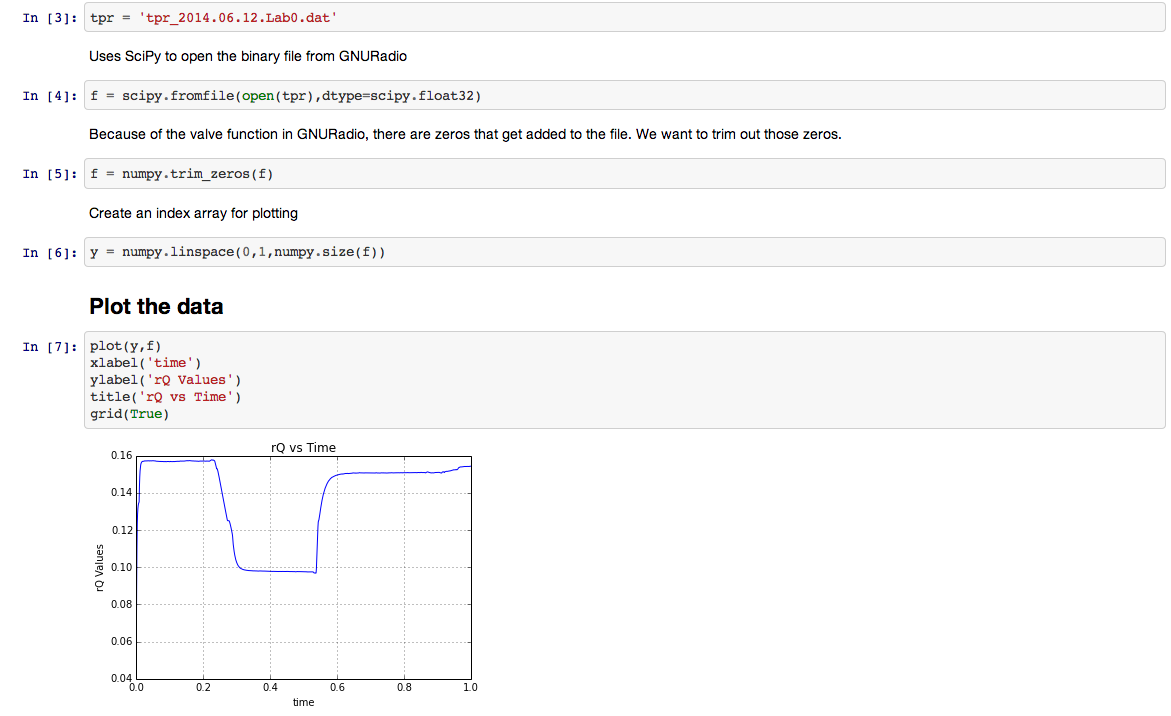
\includegraphics[width=17cm]{Images/python_gnuradio.png}
\isucaption{A screenshot showing the iPython notebook code and related graphs generated for parsing GNURadio data}
\label{matlab_display}
\end{figure}

The first data we will look at with be with the software defined radio.  The SDR records the total power measurements to a binary file that either Matlab or Python can read.  This file format is explained in section \ref{exp1_data}. Additional information on data analysis is explained in section \ref{Exp1_analysis}.  We will begin by looking at the raw total power readings which we will call raw Q values or rQ values.  These are the uncalibrated total power readings from the software defined radio.  

\begin{figure}[h!tb] \centering

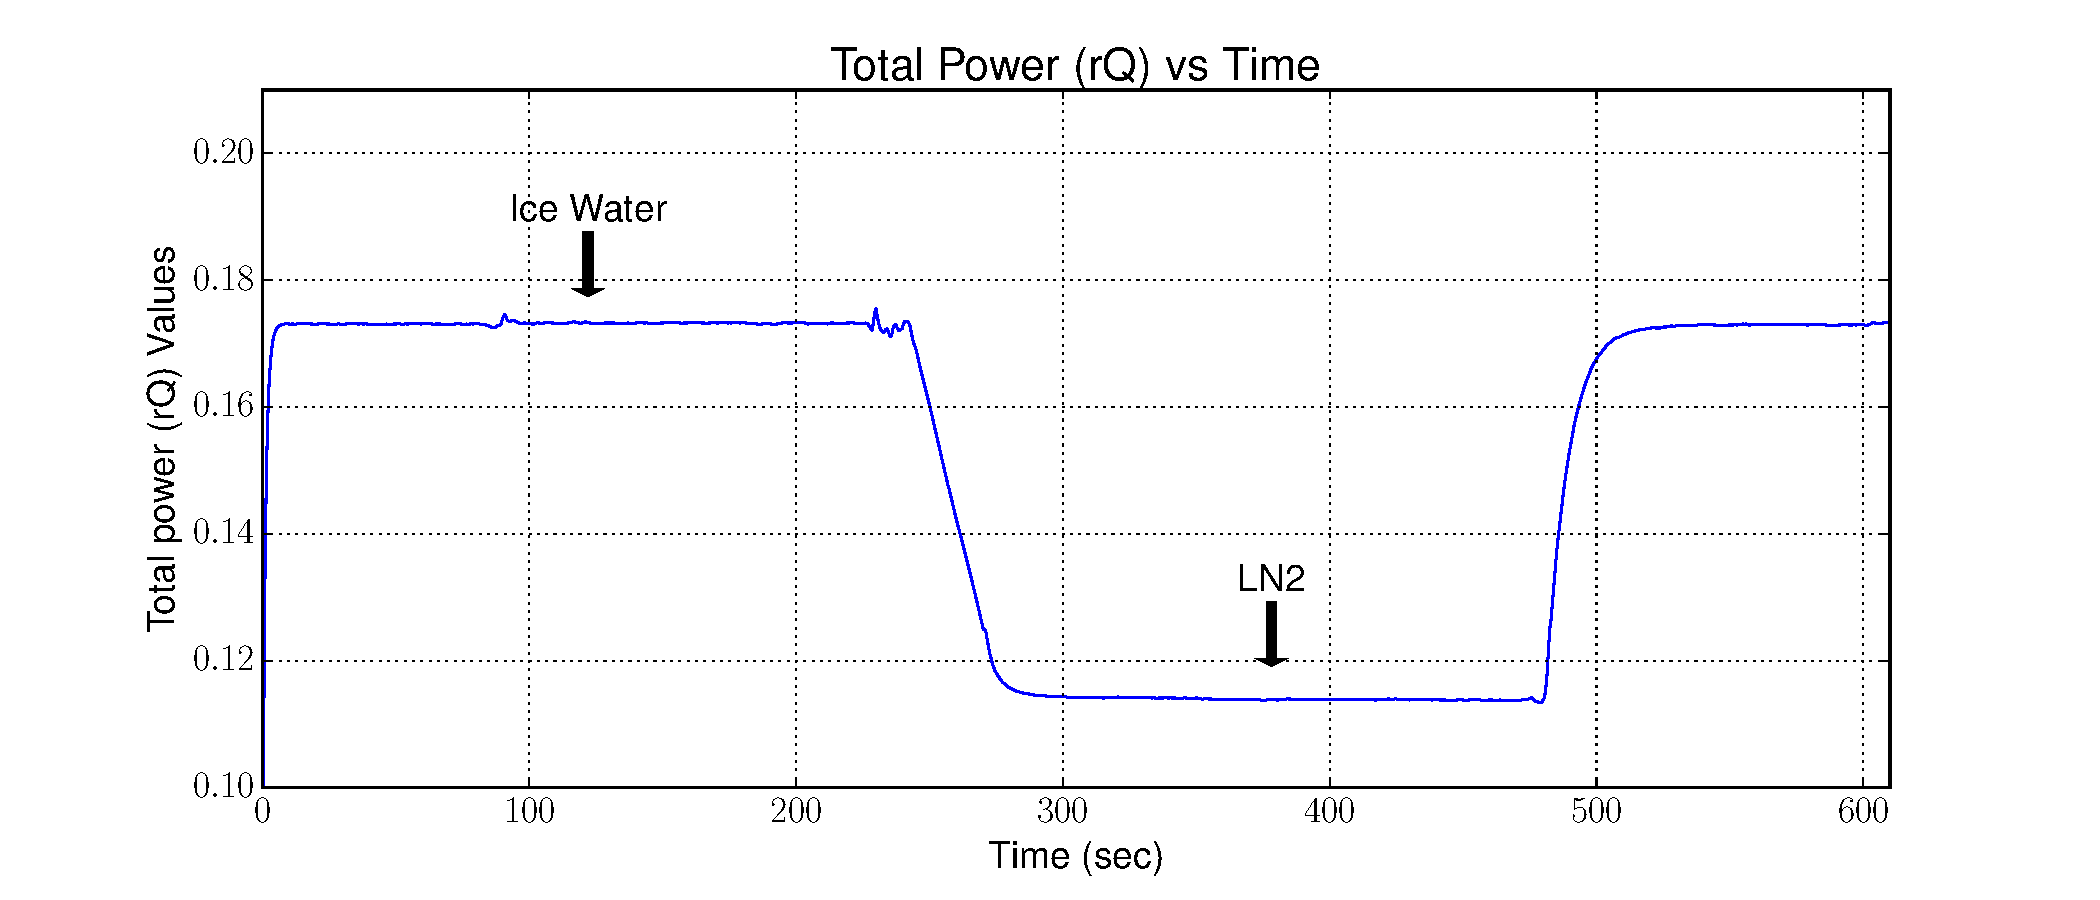
\includegraphics[width=\textwidth]{Experiments/Exp1/rqvstime_annotate.pdf}
\isucaption{Graph of the uncalibrated rQ values of Experiment I}
\label{SDR_rQ}
\end{figure}

Figure \ref{SDR_rQ} shows the total power reading versus time and is also marked when the matched load was submerged in Ice Water, LN2, or a hot water bath.  Since we know what the temperatures are for the ice water and LN2, we can now calibrate these readings to a noise temperature reading.  This is done by reading in a calibration file we have stored in csv format and performing linear algebra to solve the slope of the line.  This was done in our iPython Notebook using the following code.

\lstset{language=Python}
\begin{lstlisting}[frame=single,keywordstyle=\color{blue}]
a = numpy.array([[rQ_values[0],1.0],[rQ_values[1],1.0]],numpy.float32)
b = numpy.array([temp_values[0],temp_values[1]])
z = numpy.linalg.solve(a,b)
\end{lstlisting}

Now that we have our calibration points, we can now re-graph this data but now calibrated as a reference noise temperature. Figure \ref{SDR_Calibrated} shows a calibrated graph of the data in relation to noise temperature.  In addition, we have colorized this graph to show warmer to cooler temps.  This is helpful as we often refer to these as noise temperatures.

\begin{figure}[h!tb] \centering

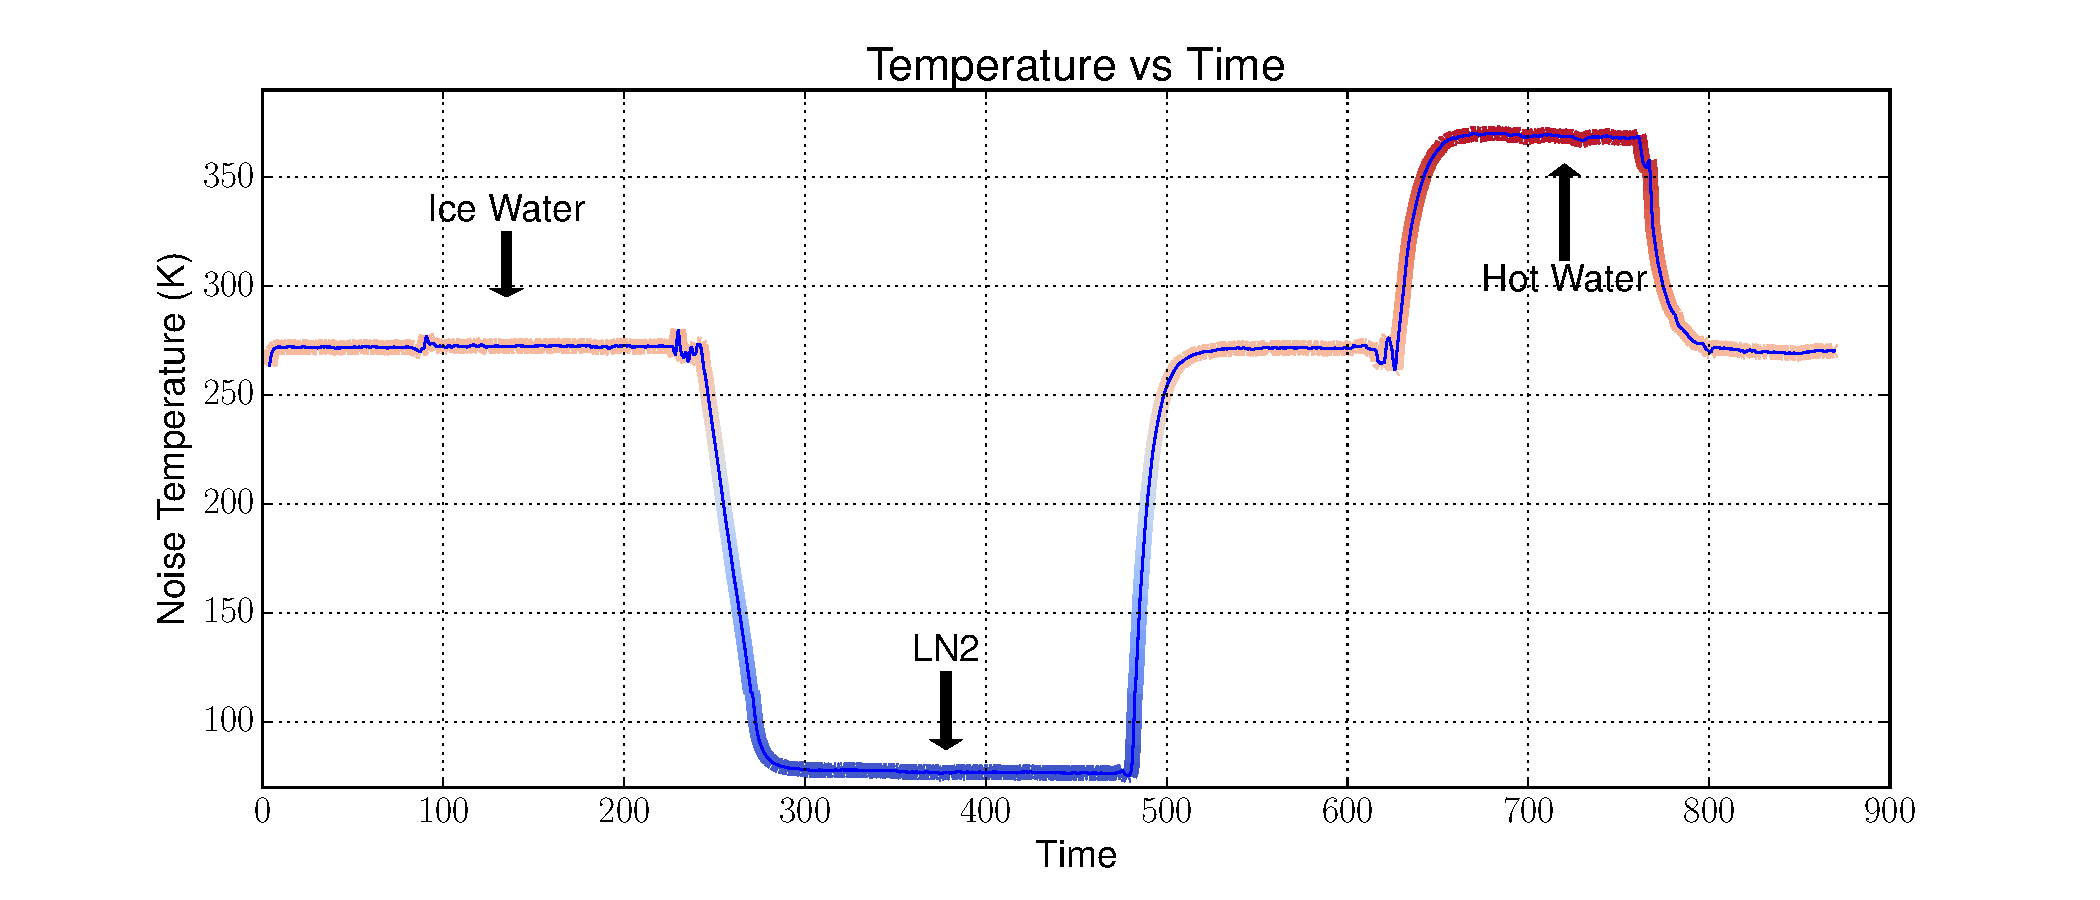
\includegraphics[width=\textwidth]{Experiments/Exp1/sdr_calibrated_color.pdf}

\isucaption{Graph of the calibrated noise temperature of Experiment I}
\label{SDR_Calibrated}
\end{figure}

Now that we have looked at the software defined radio data, we want to look at the square-law detector with the end result of comparing the two.  The square-law detector gives us power information as a voltage, so once again we will need to calibrate this to the known temperature references.  However, before that we need to do one other step with the data.  Unlike the software defined radio, there is no filter or integrator to help smooth out the data, so the square-law data is very noisy.  Our first step will be to filter the data.  Figure \ref{X2_Raw} shows our raw data that we get from the square-law detector.

\begin{figure}[h!tb] \centering
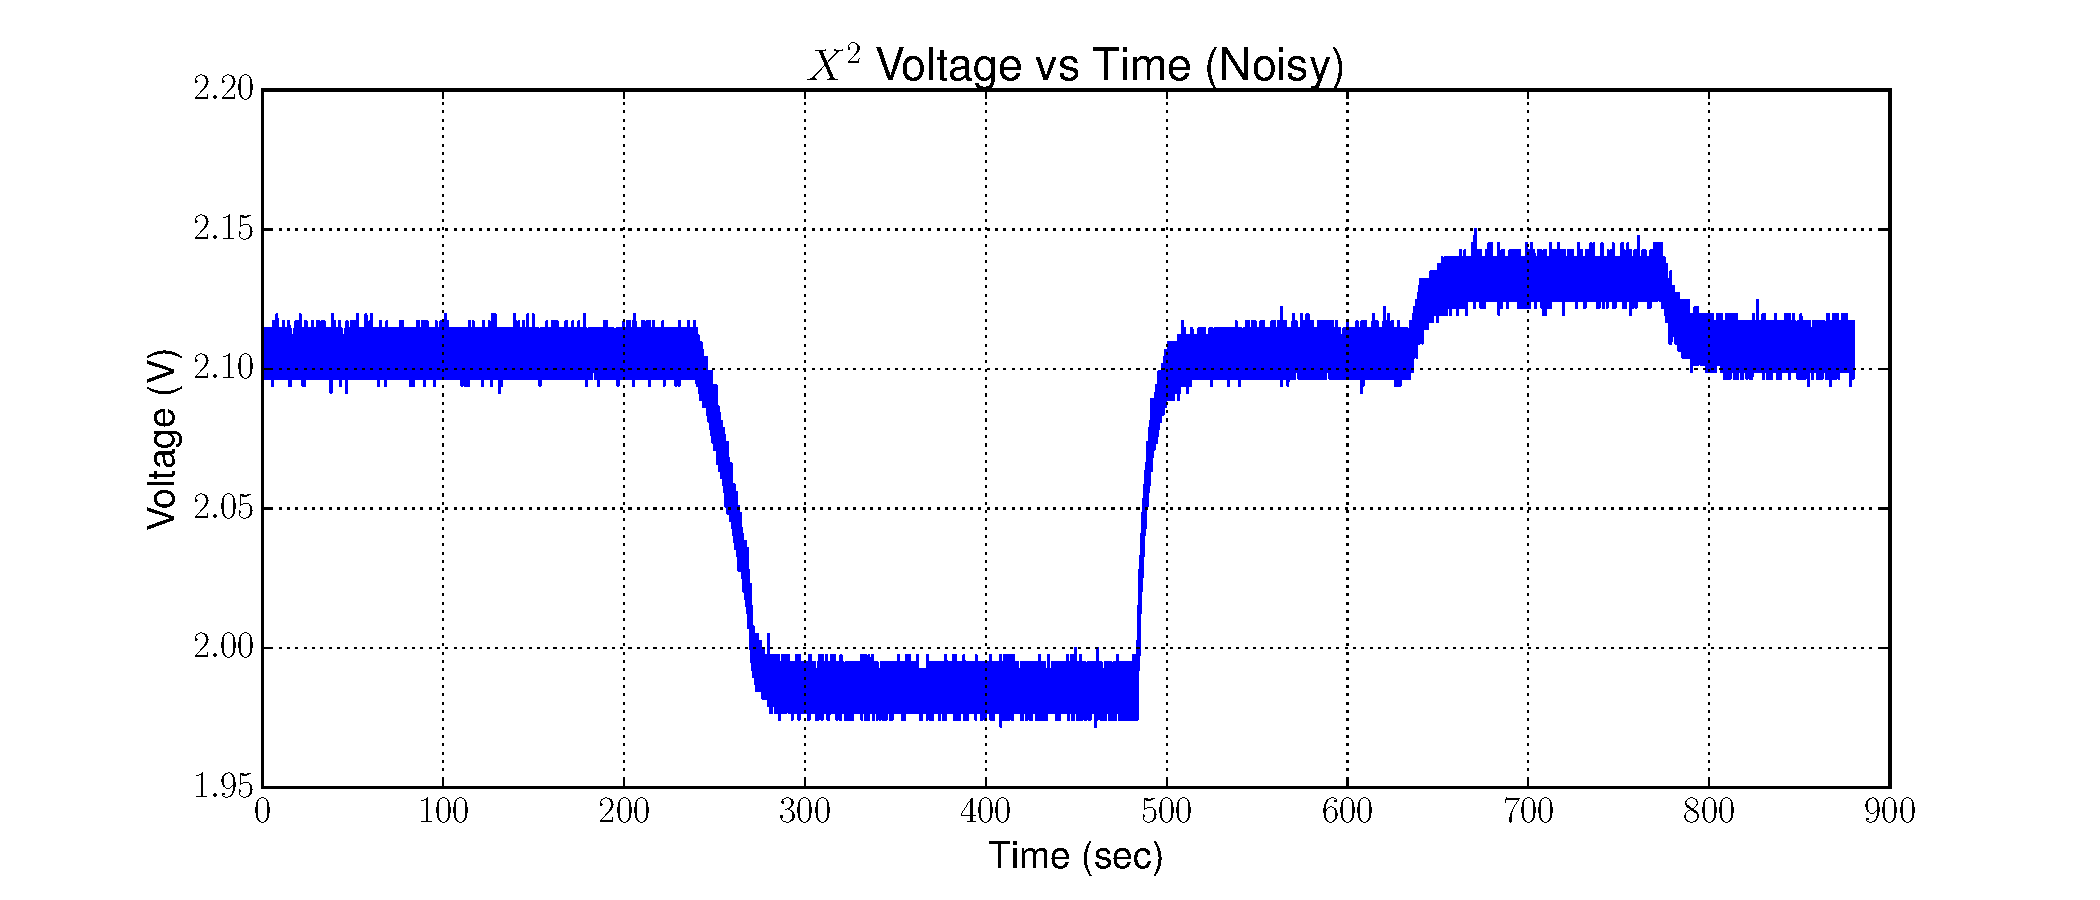
\includegraphics[width=\textwidth]{Experiments/Exp1/noisy_voltage.pdf}
\isucaption{Raw and noisy graph from the square-law detector used in Experiment I}
\label{X2_Raw}
\end{figure}

Once again we can use Python to process this information and specifically we can use SciPy which includes several useful signal processing modules.  For our use, we will use a low pass filter to clean up the signal.  The following code allows us to do just that.

\begin{lstlisting}[frame=single,keywordstyle=\color{blue}]
from scipy import signal
N=100
Fc=2000
Fs=1600
h=scipy.signal.firwin(numtaps=N, cutoff=40, nyq=Fs/2)
x2_filt=scipy.signal.lfilter(h,1.0,x2_voltage)
\end{lstlisting}

Figure \ref{X2_filter} now shows our data that has been filtered by the low pass filter.  This is similar to the low pass filter that is also used by the software defined radio.

\begin{figure}[h!tb] \centering
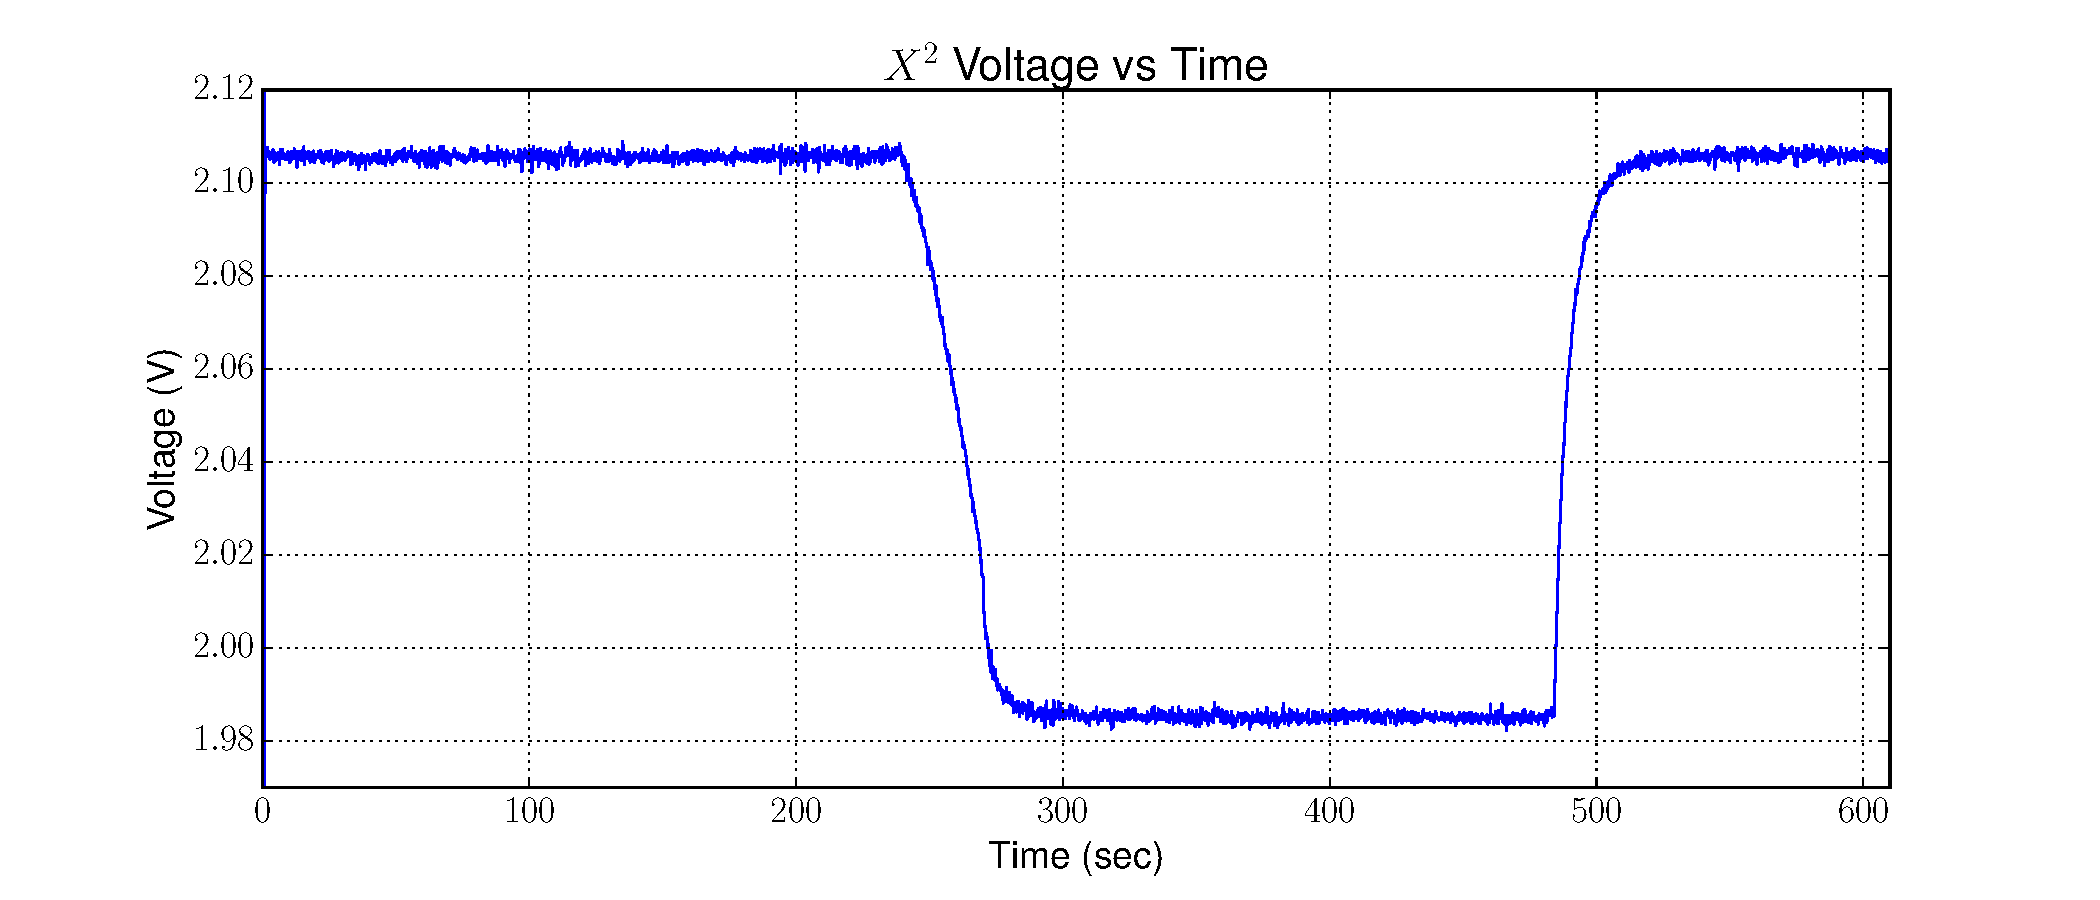
\includegraphics[width=\textwidth]{Experiments/Exp1/x2_filter.pdf}
\isucaption{Filtered data from the square-law detector used in Experiment I}
\label{X2_filter}
\end{figure}

Using the same technique as earlier, we can now calibrate the raw voltages from the square-law detector to the noise temperature.  Like the software defined radio data, we can calibrate the voltages from the square-law detector to the physical temperature that our matched load is placed in.  Figure \ref{X2_Calibrated} shows the data from the square-law detector calibrated to our known temperature points.  This now allows us to directly compare the square-law detector to the software defined radio data since we have a common reference point in which to compare the data.

\begin{figure}[h!tb] \centering
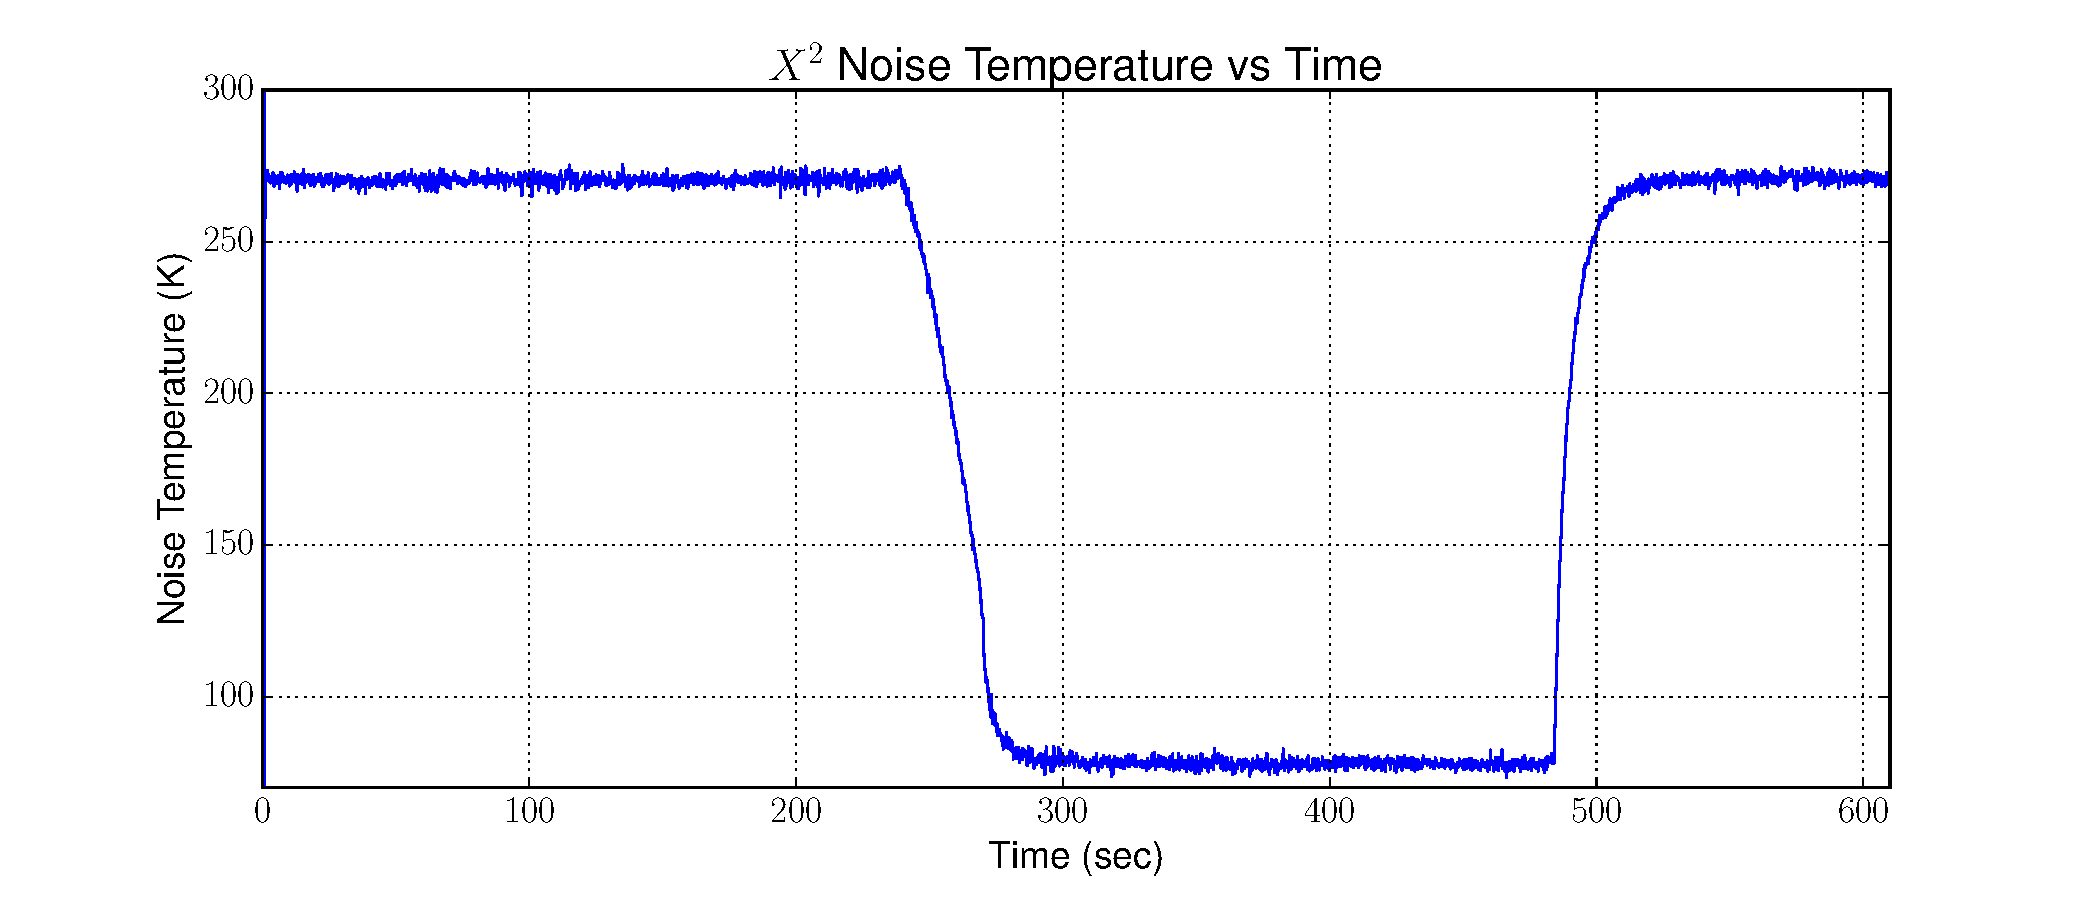
\includegraphics[width=\textwidth]{Experiments/Exp1/x2_calibrated.pdf}
\isucaption{Calibrated data from the square-law detector used in Experiment I}
\label{X2_Calibrated}
\end{figure}

We now want to compare both the Software Defined Radio and the square-law to make sure that they match up.  Since both the SDR and the square-law are now calibrated to a noise temperature, we can easily graph both of the data and compare to see how well they match up.

\begin{figure}[h!tb] \centering

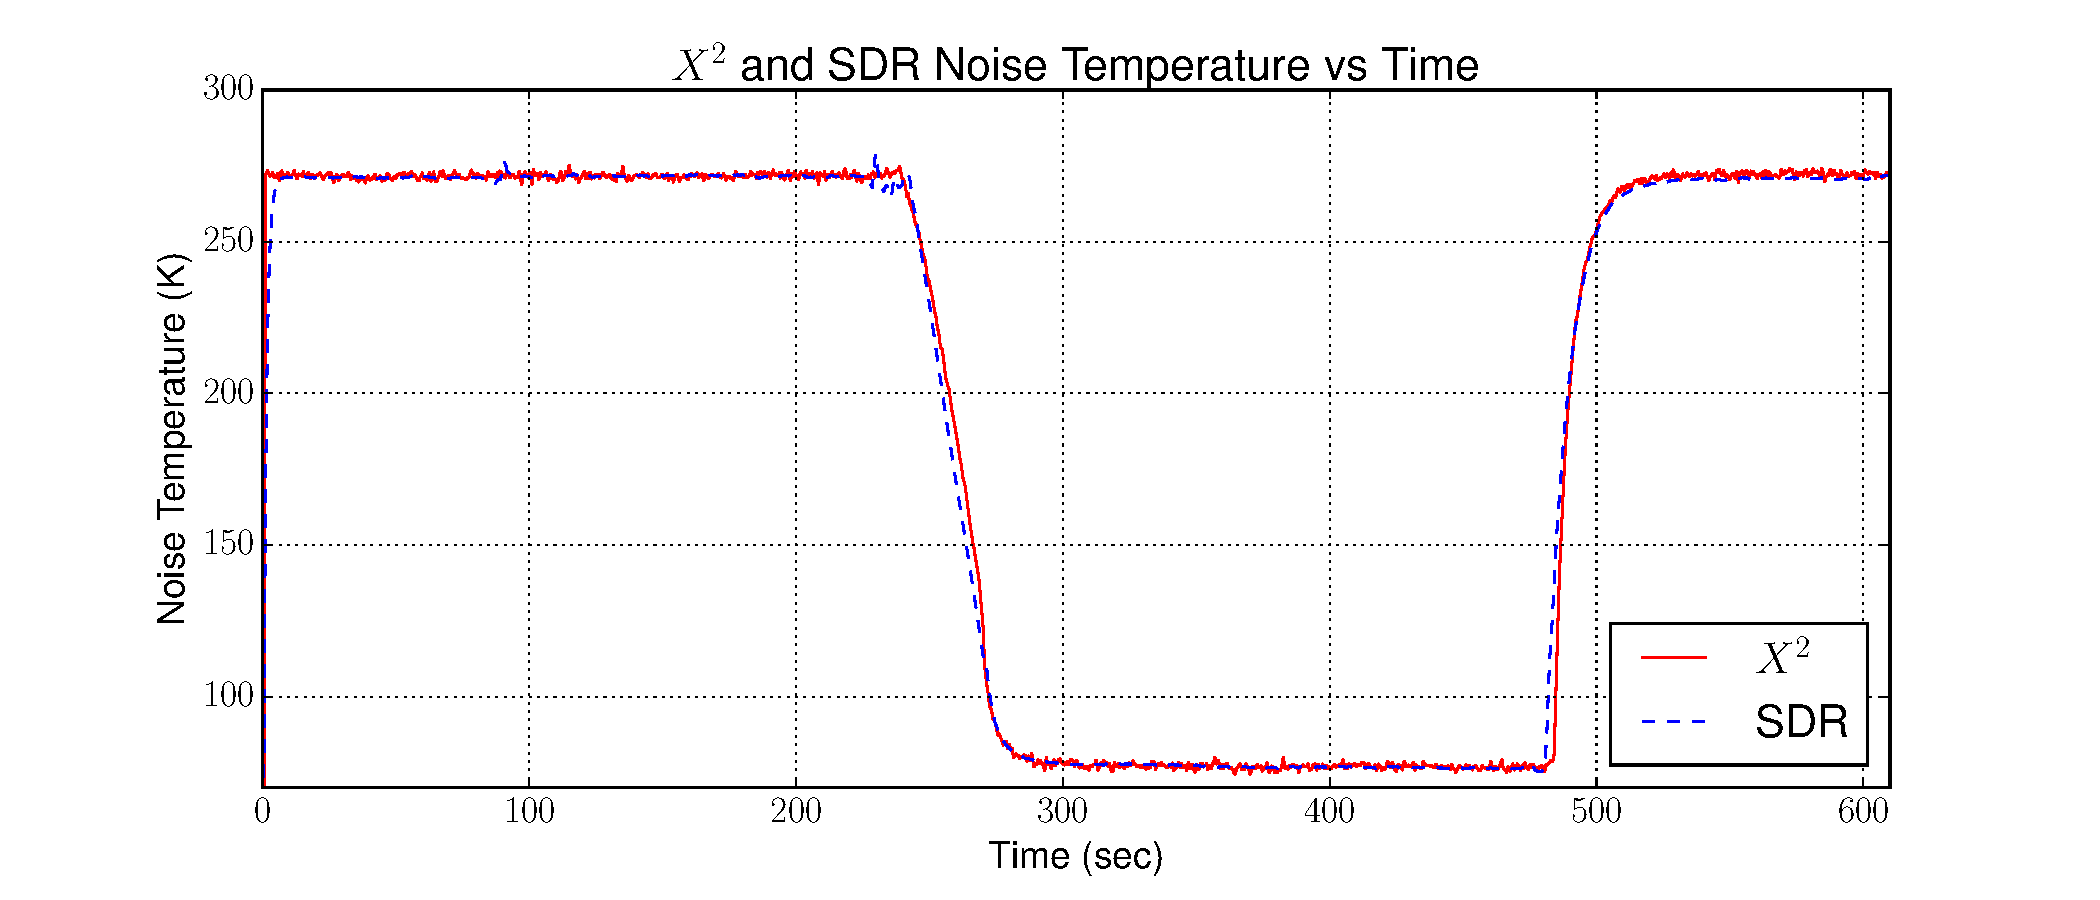
\includegraphics[width=\textwidth]{Experiments/Exp1/x2_SDR_Calibrated.pdf}
\isucaption{Figure showing both the SDR and square-law noise temperature data in Experiment I}
\label{X2_SDR_Both}
\end{figure}

We can see in Figure \ref{X2_SDR_Both} that both the software defined radio and the square-law detector match up very nicely.  This shows that both the square-law detector and the software defined radio agree when properly calibrated.  This verifies that the software defined radio can indeed operate as a total power radiometer and the data we obtain from this setup agrees with an analog and more traditional radiometer.

For the data analysis in this experiment, the data collected from the software defined radiometer was compared with a known method of collecting total power readings by using a square-law detector.  The analysis of this data showed that the calibrated information from both the software defined radiometer and the square-law detector matched up.  This proved that the software defined radiometer was indeed performing as expected for a radiometer.  It also demonstrated that calibration is possible using two reference temperatures.  

Further analysis was then conducted to compare how a software defined radiometer might be used in a typical application, such as soil moisture measurements.  This is covered in the next section.

\subsection{Application with Soil Moisture Readings}
A common application of radiometers is in the measurement of soil moisture.  All items naturally emit RF energy due to the random excitation by the electrons in the object.  The amount of noise that gets generated varies by temperature, but the amount that reaches the antenna varies by the amount of moisture in the soil.  If we can calibrate the radiometer to two known soil conditions, then we can measure the various levels of soil moisture in the soil.  At this time, we will simply look at the percentage of moisture in the soil, which will vary from zero percent or dry soil to one hundred percent or very wet soil.  The drier the soil, the more thermal noise we receive and the "warmer" the noise temperature.  Wet soil on the other hand attenuates the thermal noise and shows up as a "cooler" noise temperature.  

Using the Software Defined Radio, we can set up two methods to visually look at the noise temperature and thus the soil moisture percentage.  Since we do not have an antenna hooked up, we will simulate this by using two reference temperatures.  In this case the ice water bath and the LN2 that we just used and was shown earlier.  

A unique visual aid we can use with GNURadio is a waterfall display.  This display gives us information that includes frequency, amplitude and time.  It is referred to as a waterfall display due to the fact the display continually moves from top to bottom and looks like a waterfall.  Amplitude information is given by mapping the range of amplitudes to a color bar.  Frequency is given on the x-axis and time is on the y-axis.  Figure \ref{LN2_waterfall} shows a screen shot of the waterfall display in the GUI created in GNURadio Companion for this experiment.  This is the same program we have used but with the waterfall display now added.  The data for the waterfall is pulled directly from our source block or in our case the N200 software defined radio.

\begin{figure}[h!tb] \centering

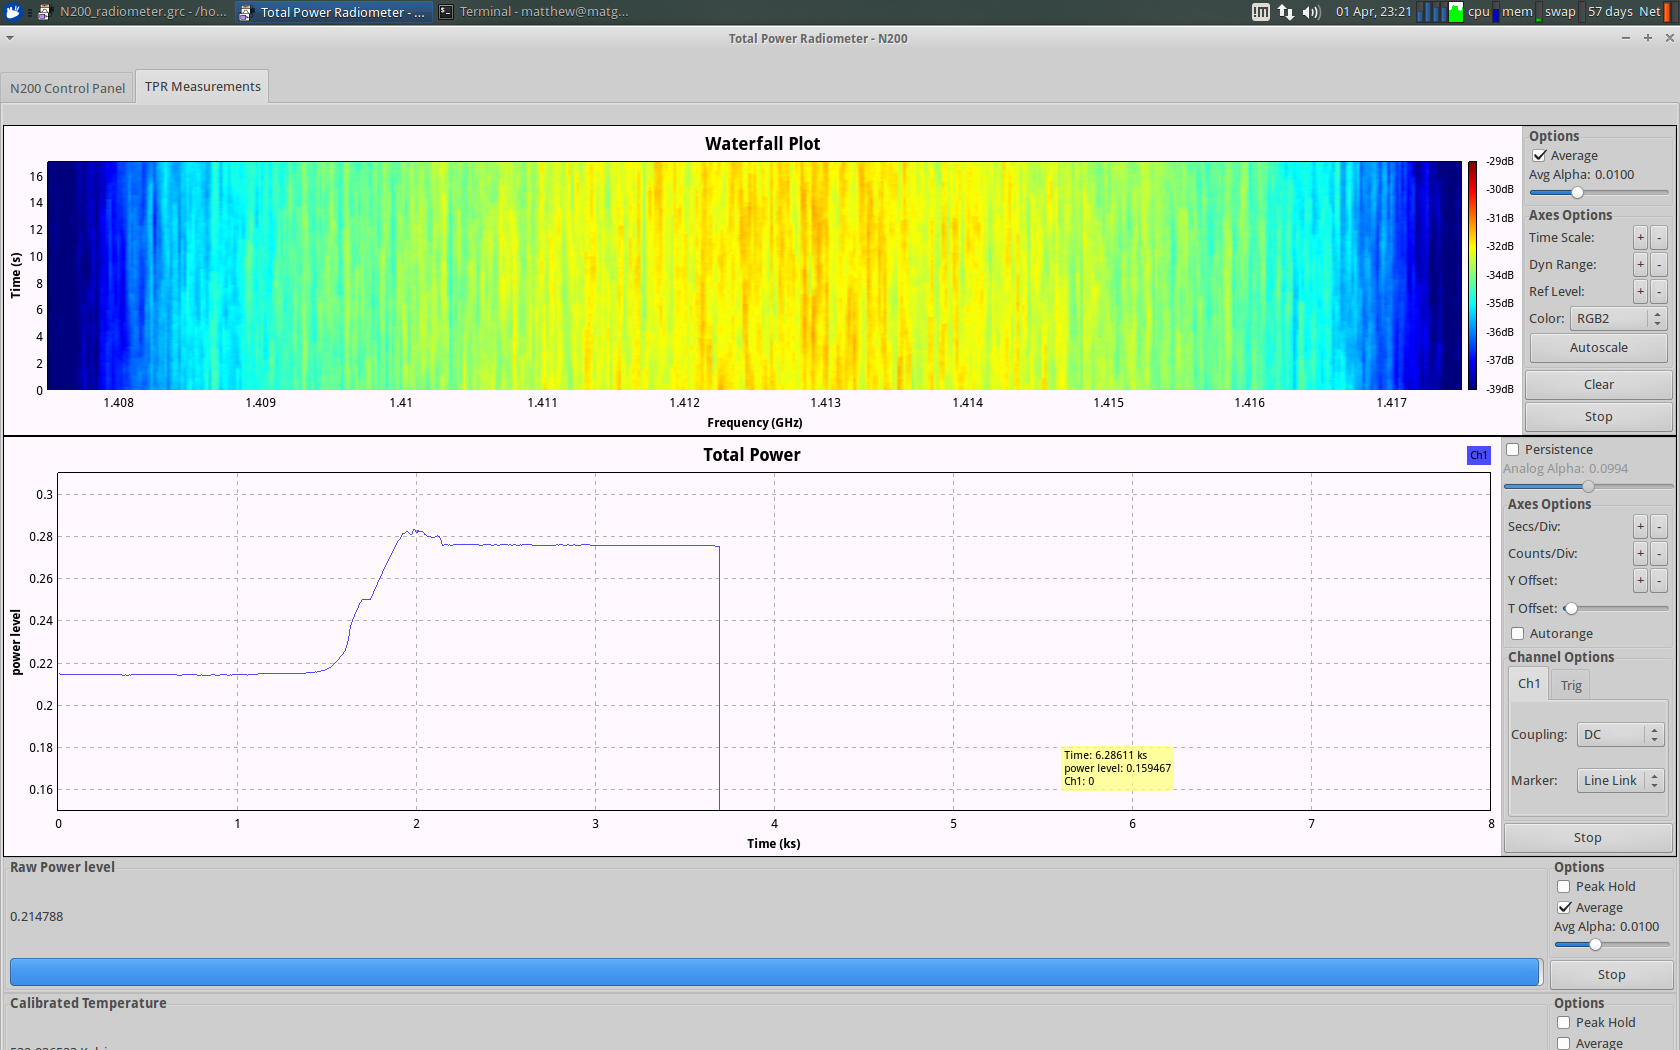
\includegraphics[width=\textwidth]{Experiments/Exp1/LN2_waterfall.png}

\isucaption{Screenshot of the waterfall display used in Experiment I}
\label{LN2_waterfall}
\end{figure}

Let's take a look at two screen shots of the waterfall.  We will put them side by side so we can better compare the display when the thermal load is in the ice water bath and when the load is in LN2.

\begin{figure}[h!tb] \centering

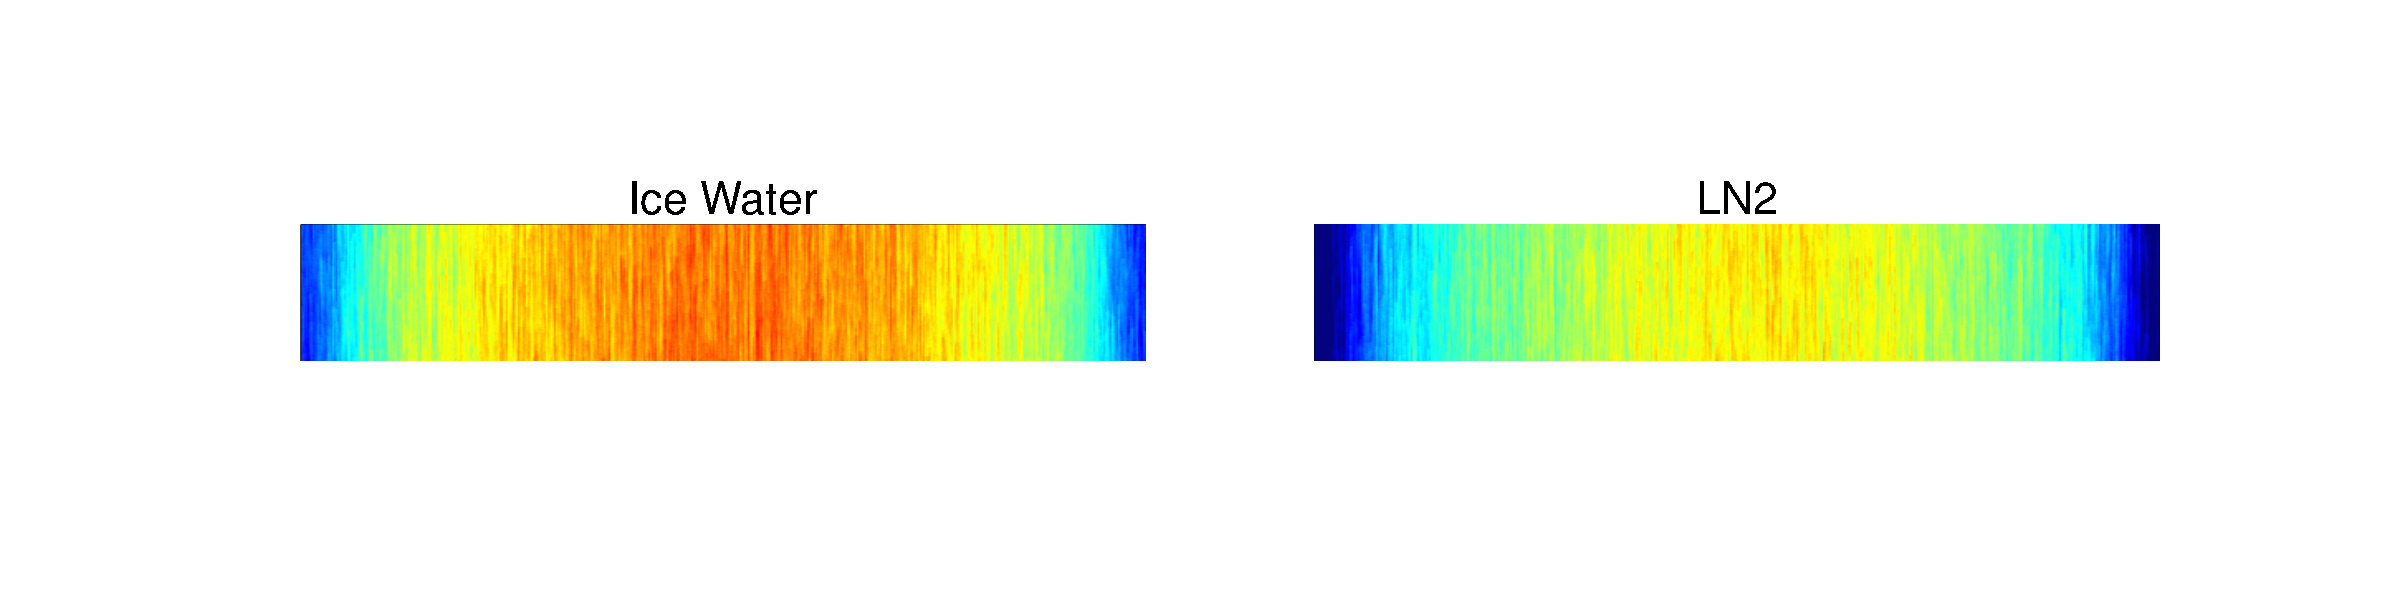
\includegraphics[width=\textwidth]{Experiments/Exp1/waterfall_side.pdf}

\isucaption{Side by side comparison of the waterfall display for Experiment 1}
\label{side_waterfall}
\end{figure}

In figure \ref{side_waterfall} we can see that the ice water screen shot appears warmer than the right side screen shot which appears cooler.  There is a limitation in GNURadio and the waterfall display that limits what the range for the power readings are.  The overall power that we see only changes by about 3 dB and our current range in the waterfall display is set to 10 dB.  If we could reduce the range, the color change would be even greater and more pronounced.  However, this does show that a change can be seen visually with color to indicate the noise temperature.  

If we assume that our LN2 is dry soil and that our ice water bath is wet soil, we can now interpolate the data to this scale and show the information we obtained in Experiment one as both a noise temperature and soil moisture.  Figure \ref{SDR_soil} shows the same data we looked at earlier but we have now added a scale to show soil moisture as a percentage.

\begin{figure}[h!tb] \centering

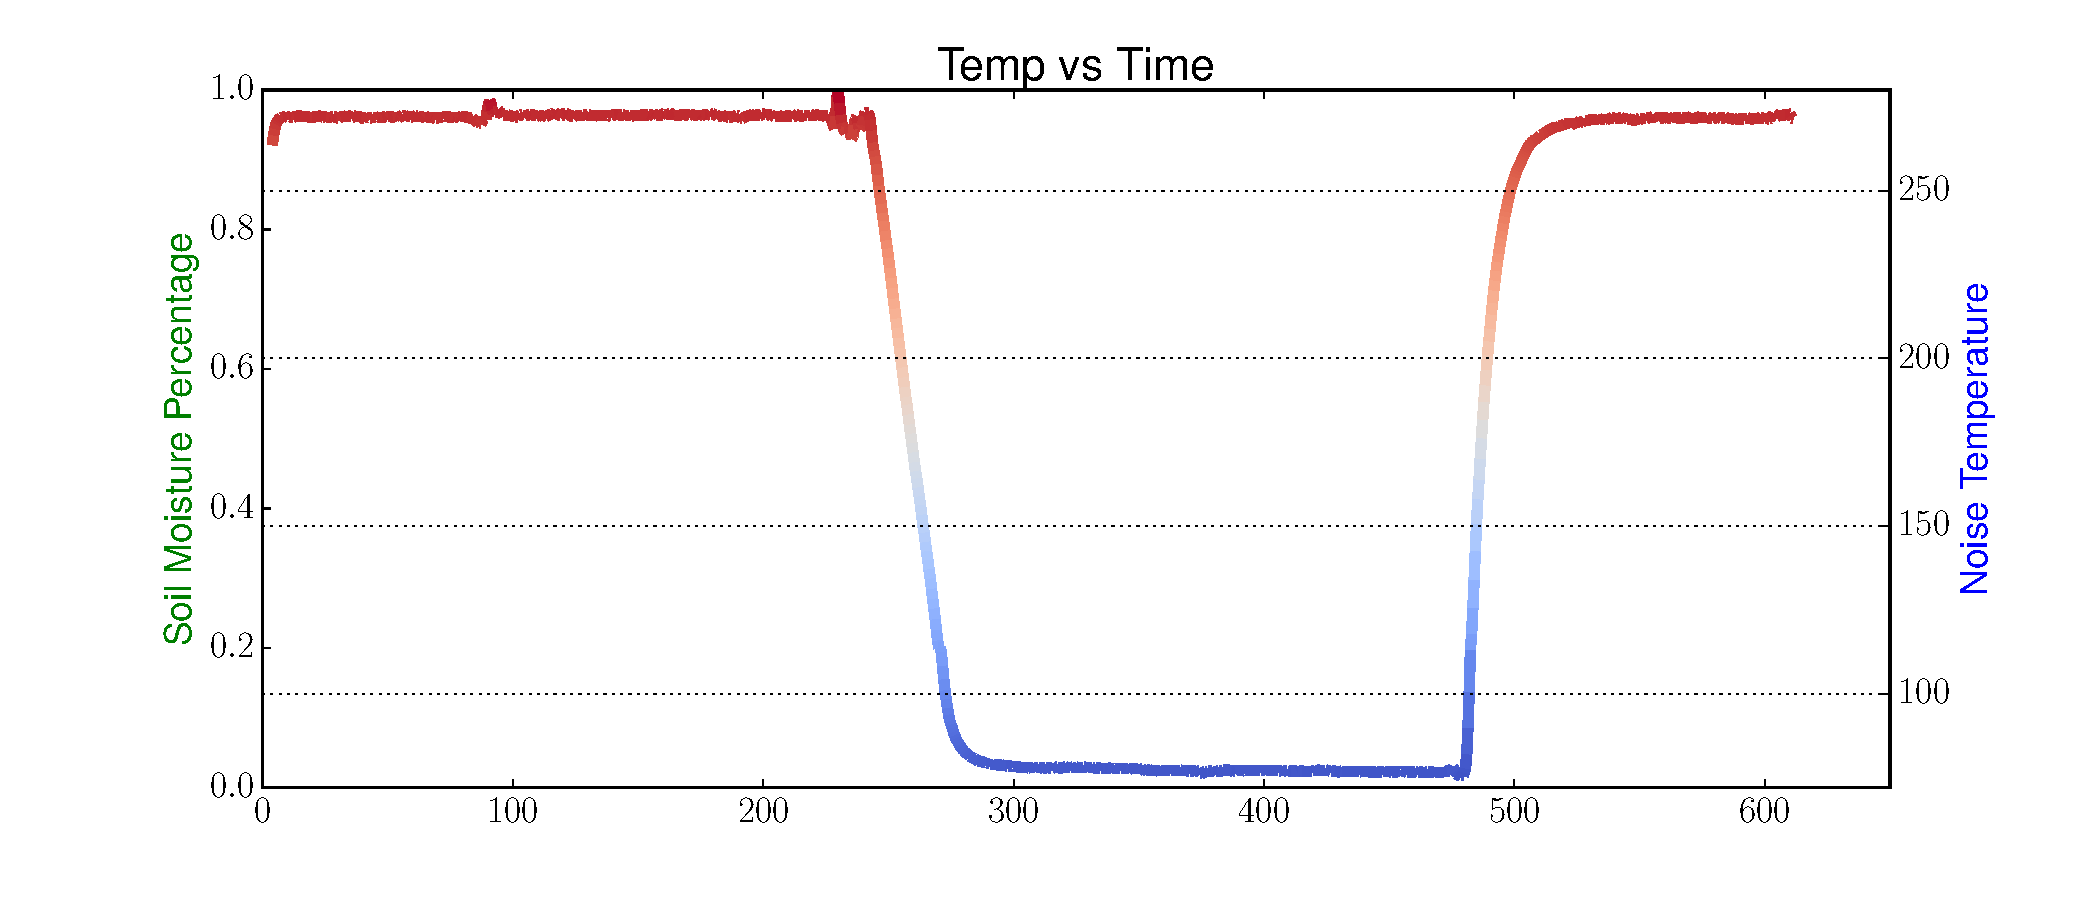
\includegraphics[width=\textwidth]{Experiments/Exp1/sdr_soilmoisture.pdf}
\isucaption{Plot of the noise temperature of Experiment 1 with soil moisture percentage}
\label{SDR_soil}
\end{figure}

While this demonstrates that we can calibrate our total power readings with a soil moisture percentage, we would use actual field tests to calibrate the radiometer.  In addition, we could also calibrate to soil moisture content instead of a percentage if desired.  Both methods have been done with traditional radiometers[\cite{Jonard}][\cite{Shi}.

\section{Experiment II - Verification of sensitivity and stability} \label{Exp2_results}

\subsection{Data Collected}
For the sensitivity portion of this experiment, the same data collected from section \ref{Exp1_data} is used.  The data collected for the stability is the total power data collected from the software defined radiometer. For calibration the data points shown in table \ref{exp2_datapoints} was collected and used to calibrate the total power measurements.

\begin{table}[h!tb] \centering
\isucaption{Total Power calibration data points for the stability experiment}
\label{exp2_datapoints}
% Use: \begin{tabular{|lc|} to put table in a box
\begin{tabular}{lc} \hline
\textbf{rQ Value} & \textbf{Temperature (K)} \\ \hline
.1132 & 77 \\
.1770 & 271.65 \\ \hline
\end{tabular}
\end{table}
 
\subsection{Data Analysis}\label{Exp2_analysis}

\emph{Sensitivity.}  Sensitivity for a radiometer is the $NE\Delta T$ that was covered in chapter \ref{ch:background} and specifically can be found in equation \ref{NEAT_EQ}.  This $NE\Delta T$ is also the standard deviation of the data that we collect from the software defined radiometer.  

The standard deviation is calculated to be 0.09 Kelvin by using the standard deviation function found in NumPy.  We can compare this to what we expected the $NE\Delta T$ to be which uses equation \ref{NEAT_EQ}.  To calculate the $NE\Delta T$, we need to know the integration time, the bandwidth, the total system and antenna noise.  This information is found in table \ref{exp2_param}.

\begin{table}[h!tb] \centering
\isucaption{Experimental parameters for experiment one.}
\label{exp2_param}
% Use: \begin{tabular{|lcc|} to put table in a box
\begin{tabular}{ccc} \hline
\textbf{Bandwidth ($\beta$)} & \textbf{Integration Time ($\tau$)} & \textbf{$T_{A}+T_{sys}$}\\ \hline
10 MHz & 2 sec & 437 K \\ \hline
\end{tabular}
\end{table}

Python was then used to calculate the $NE\Delta T$ using the data from table \ref{exp2_param}.  The python code listed below is used to calculate the expected $NE\Delta T$.

\begin{lstlisting}[frame=single,keywordstyle=\color{blue}]
tau = 2
BSDR = 10e6
Tsys = 350
TA = 77
NEAT_SDR = (TA+Tsys)/sqrt(BSDR*tau)
\end{lstlisting}

This gives us the result of 0.1 Kelvin for the expected $NE\Delta T$.  We can now look at the data collected from experiment one.  Since the sensitivity is related to the standard deviation of the graph, we can use Python to give us the standard deviation of the data.  To determine our sensitivity, we will zoom in on data that was collected while the matched load was submerged in LN2.  Figure \ref{Sensitivity} shows this graph.  

\begin{figure}[h!tb] \centering
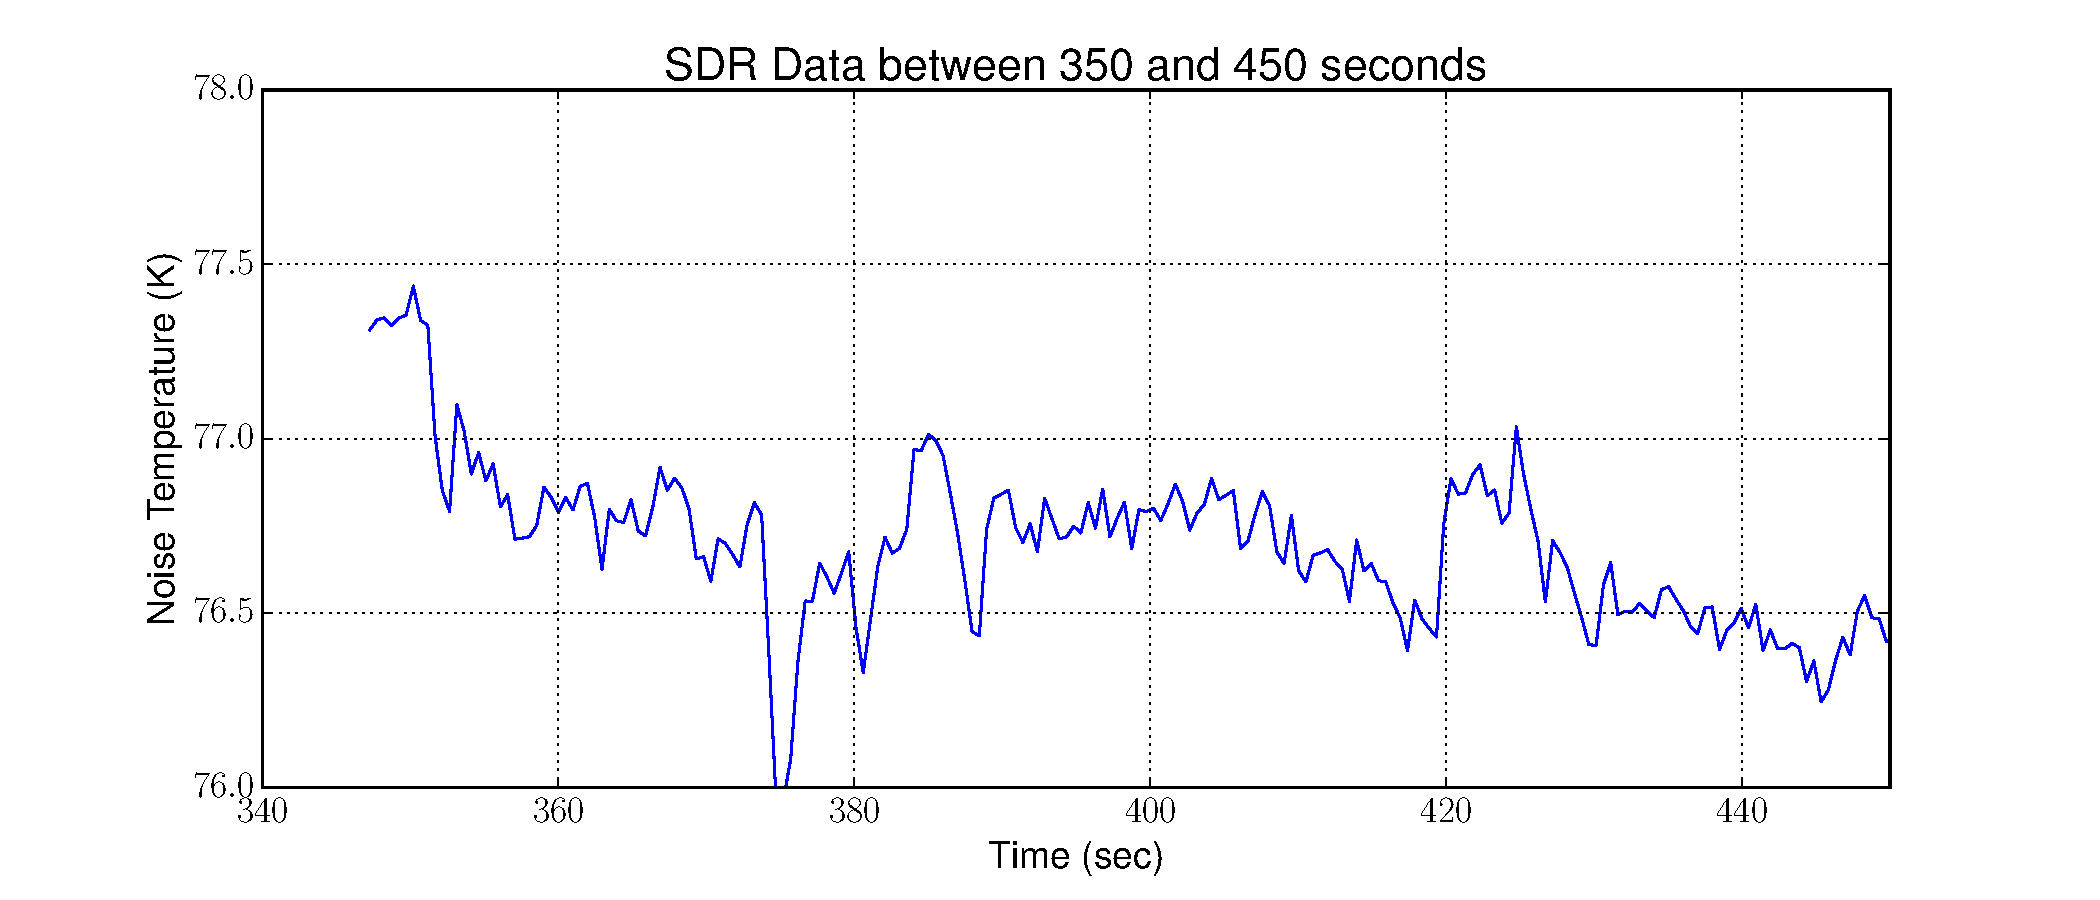
\includegraphics[width=\textwidth]{Experiments/Exp1/SDR_Zoom.pdf}
\isucaption{Graph of the calibrated total power from experiment one while submerged in LN2.}
\label{Sensitivity}
\end{figure}

Using Python we can determine the standard deviation of this range of data.  Using Python, we find that the standard deviation for this section of data is .23 Kelvin.  We can now plot both the expected sensitivity and the actual sensitivity which is shown in figure \ref{sensitivity_exp_real}.

\begin{figure}[h!tb] \centering
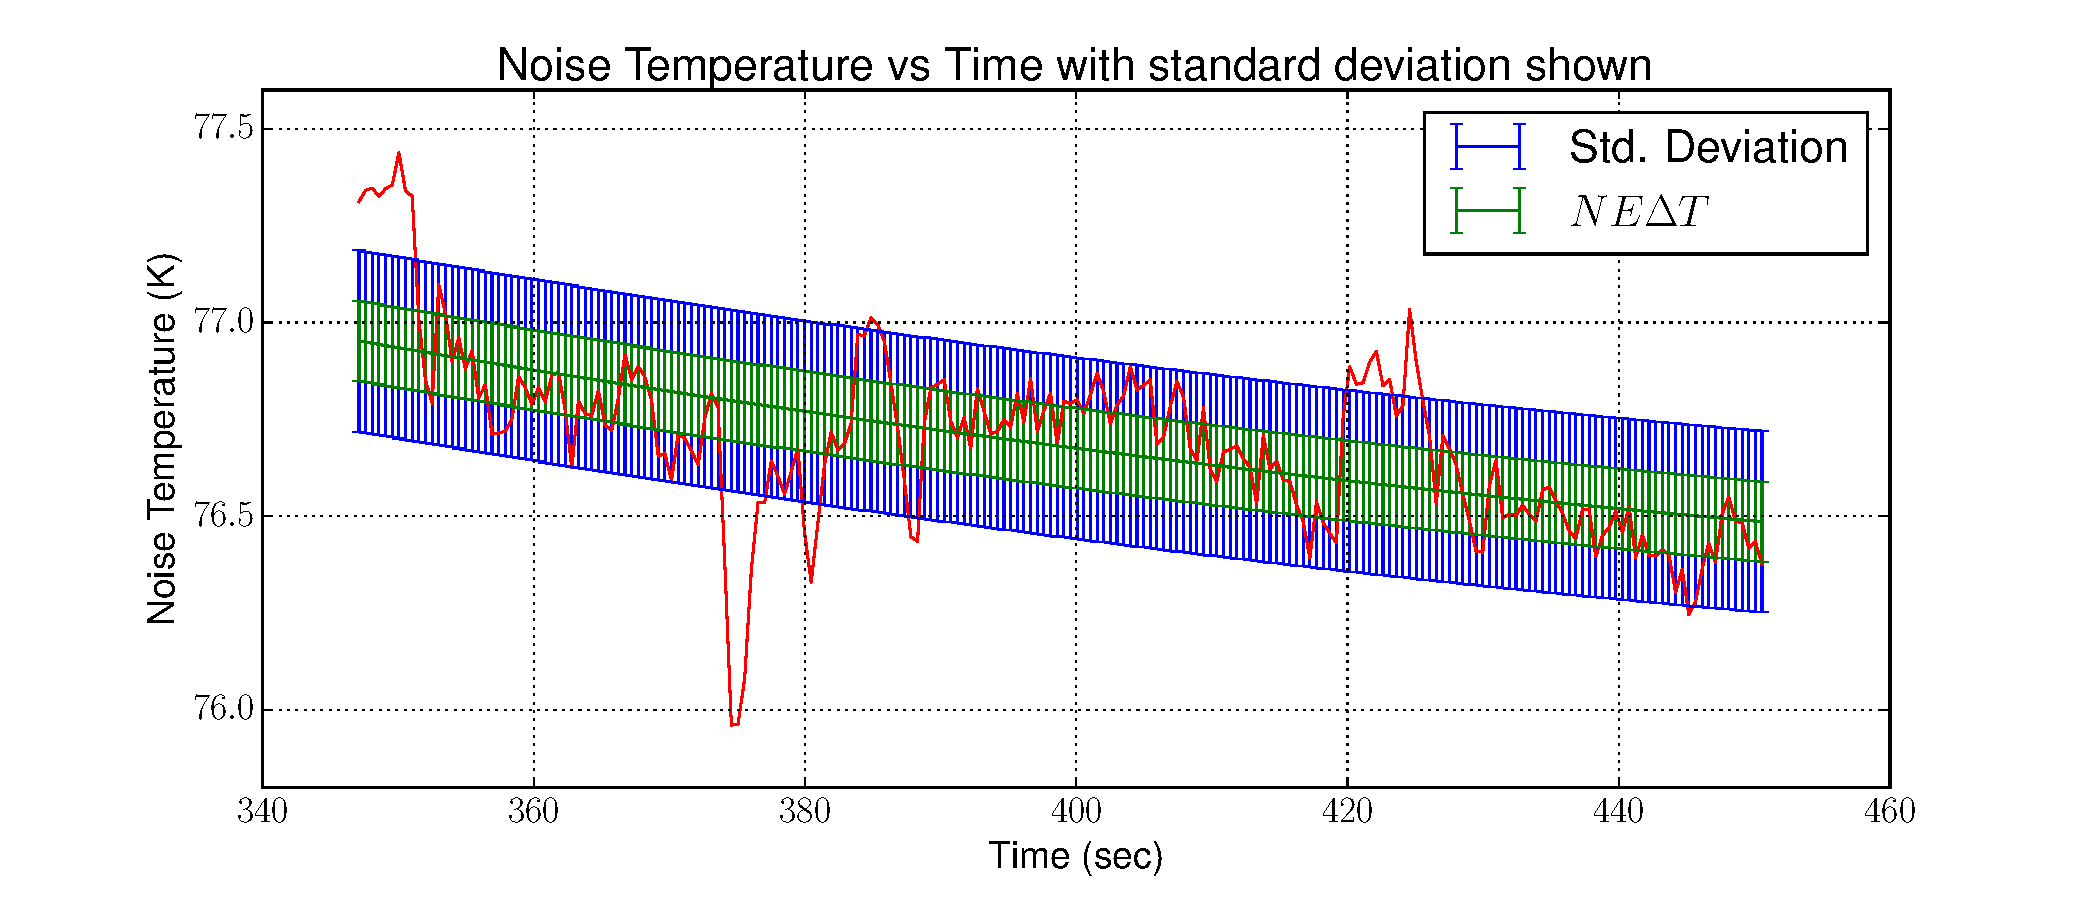
\includegraphics[width=\textwidth]{Experiments/Exp1/std_dev_errbar.pdf}
\isucaption{Graph of the calibrated total power with expected and actual sensitivity.}
\label{sensitivity_exp_real}
\end{figure}

While .23 Kelvin is higher than the calculated sensitivity, it is still quite acceptable.  As discussed in chapter \ref{ch:implementation} and shown in table \ref{rad_performance}, our target $NE\Delta T$ is one Kelvin or less.  Therefore our actual performance of .23 Kelvin still meets our requirements for a radiometer.

\emph{Stability.}  To verify stability of the radiometer, we look to see how much change the radiometer records over a relatively long period of time.  To test this a matched load was submerged in a liquid nitrogen bath for an extended period of time, in this case for fifteen minutes.  The readings were then looked at to study the trend of the data.  The data is graphed in figure \ref{Stability}.

\begin{figure}[h!tb] \centering
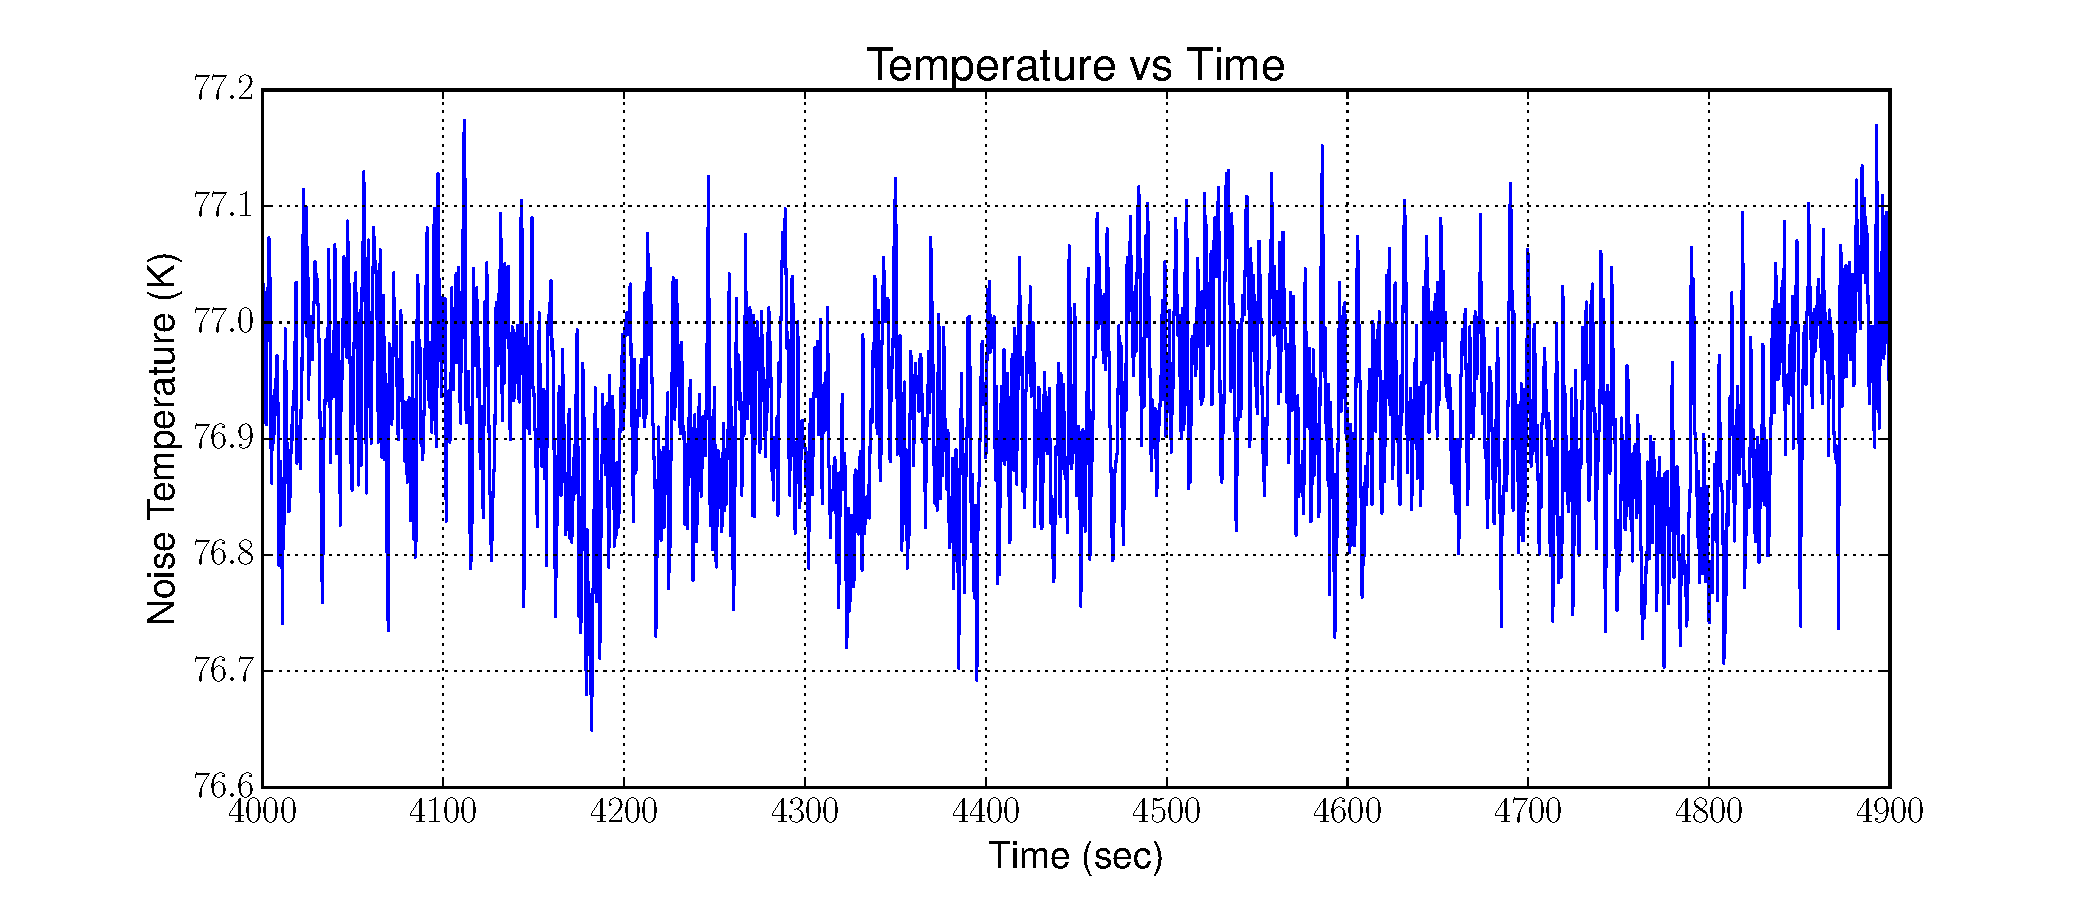
\includegraphics[width=\textwidth]{Experiments/Exp2/sdr_calibrated_zoom.pdf}
\isucaption{Graph of the calibrated total power over a period of fifteen minutes.}
\label{Stability}
\end{figure}

Once again we can look at the standard deviation to see how much of a change occurs over this time period.  

Figure \ref{Stability_calib} now shows the stability plot with both the actual $NE\Delta T$ which is the standard deviation of the graph, and the calculated $NE\Delta T$.

\begin{figure}[h!tb] \centering
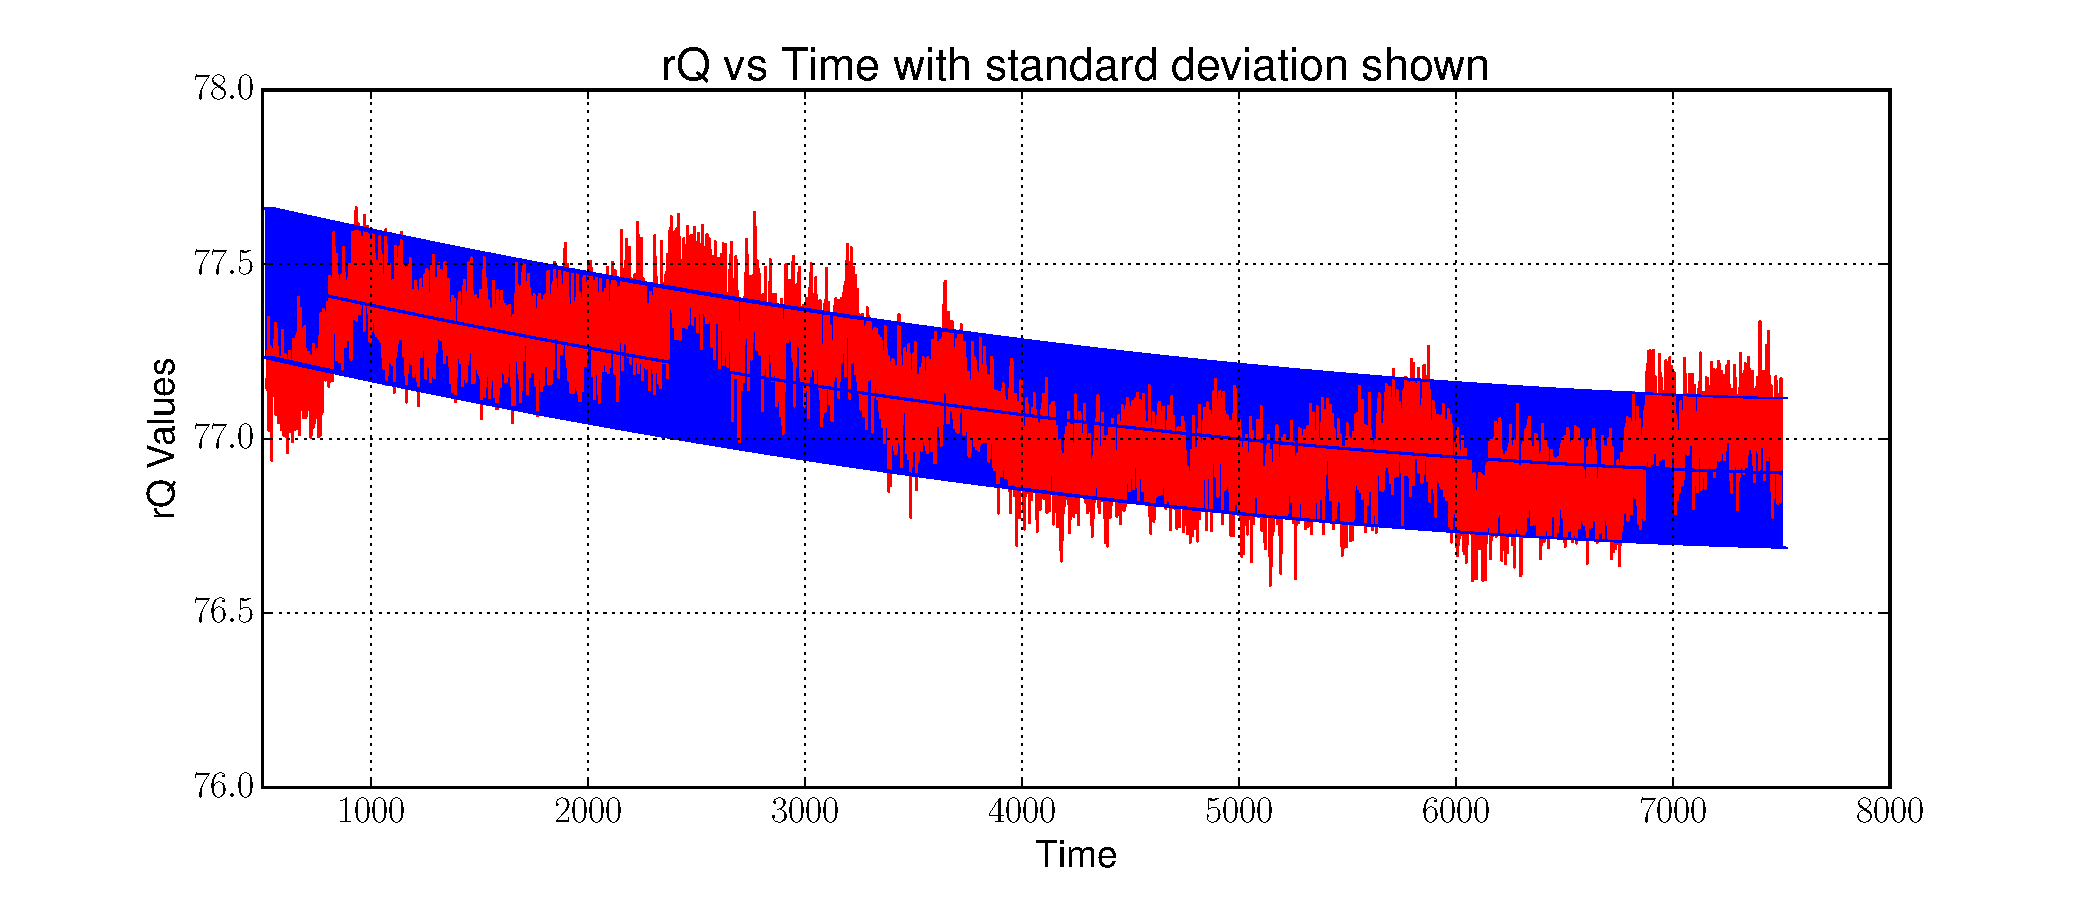
\includegraphics[width=\textwidth]{Experiments/Exp2/calib_vstime_stddev.pdf}
\isucaption{Graph of the calibrated total power with the standard deviation plotted.}
\label{Stability_calib}
\end{figure}

%As it can be seen in figure \ref{Stability}, the amount of change over a period of one hour is quite small.  The standard deviation for this sample is 0.09 kelvin.  The $NE\Delta T$ calculated using 10 MHz for the bandwidth, an integration time of 2 seconds and with our sample at 77 Kelvin is calculated to be 0.10 Kelvin with a system temperature of 350 Kelvin.  Therefore, our system is behaving as we expect it to for this stability test.

%Figure \ref{Stability_calib} shows a graph of the total readings but with the standard deviation now plotted.  This shows that the system is stable and is operating as expected within our expected $NE\Delta T$.

\section{Experiment III - Interfering Signal Mitigation} \label{Exp3_results}

The addition of an interfering signal is unwanted to the radiometer and has an adverse effect on how the radiometer operates but is a growing problem for all radiometers [\cite{Ellingson}].  This problem becomes even a greater issue with radiometers used in orbiting spacecrafts as they are able to see large areas[\cite{DeRooRFI}].  Even though the band we are working in of 1.4 GHz is an internationally protected frequency, there can still be both intentional and unintentional radiators that cause interference.

RFI detection and mitigation is not a new topic in radiometry and there have been other methods in both the detection and mitigation of these signals [\cite{Forte}][\cite{McIntyre_RFI}] [\cite{DeRoo}].

\subsection{Data Collected}

The data collected for experiment three is the total power values from the software defined radiometer and also the voltage data from the square-law detector.  These values are calibrated using the data points provided in table \ref{exp3_datapoints}.

\begin{table}[h!tb] \centering
\isucaption{Total Power calibration data points}
\label{exp3_datapoints}
% Use: \begin{tabular{|lcc|} to put table in a box
\begin{tabular}{lcc} \hline
\textbf{rQ Value} & \textbf{$X^2$ Voltage (V)} & \textbf{Temperature (K)} \\ \hline
.0361 & 2.1234 & 77 \\
.0623 & 2.1872 & 271.65 \\ \hline
\end{tabular}
\end{table}

\subsection{Data Analysis}

We begin by looking at the what happens to our total power readings with no filter applied.  As we stated in Chapter \ref{ch:exp_design}, section \ref{exp3_setup}, the frequency of the offending signal will not change, but the amplitude will.  This will mean that we should see clear indications of the total power changing as the amplitude of the offending signal changes.  

\begin{figure}[h!tb] \centering
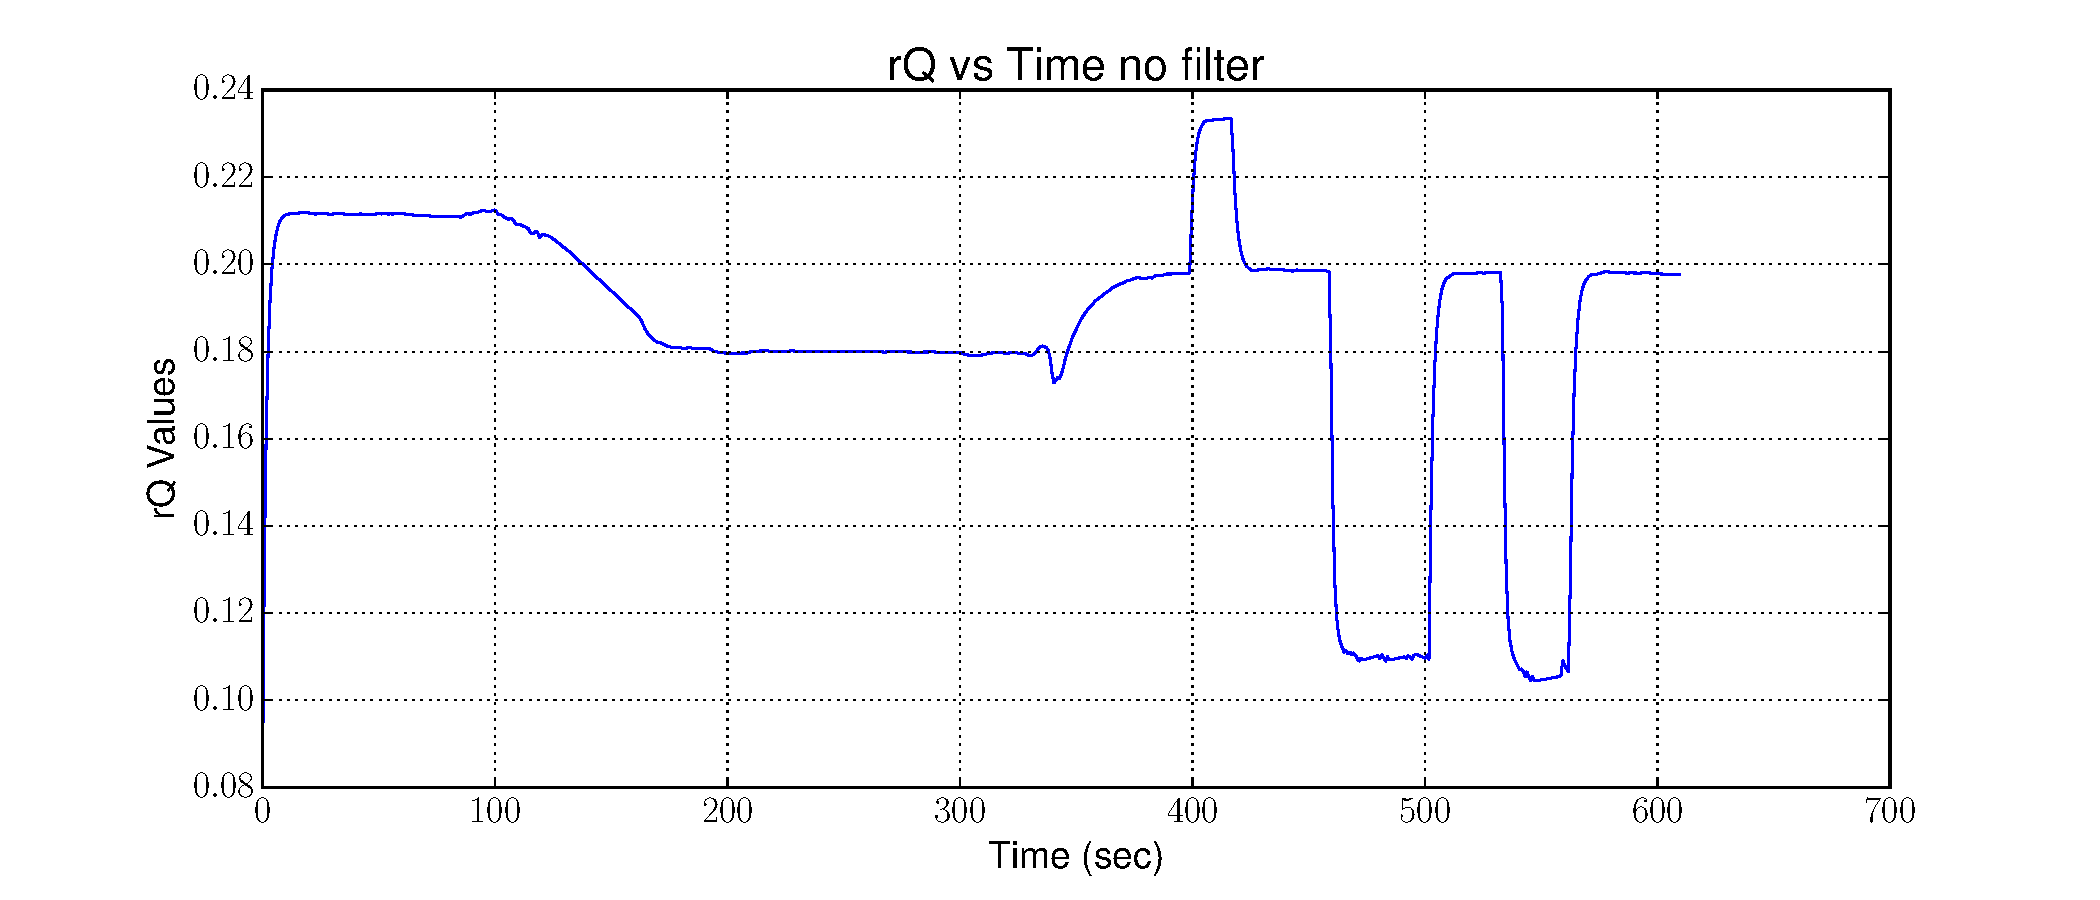
\includegraphics[width=\textwidth]{Experiments/Exp4/sdr_raw_unfiltered.pdf}
\isucaption{Graph showing the unfiltered total power measurements on the software defined radio}
\label{sdr_unfilt_raw}
\end{figure}

We can see that there are pulses that occur in the graph in figure \ref{sdr_unfilt_raw} and that changes in the amplitude of the offending signal affect our total power readings.  These same pulses can also be seen in the square-law detector data as well which can be seen in figure \ref{x2_unfilt}.

\begin{figure}[h!tb] \centering
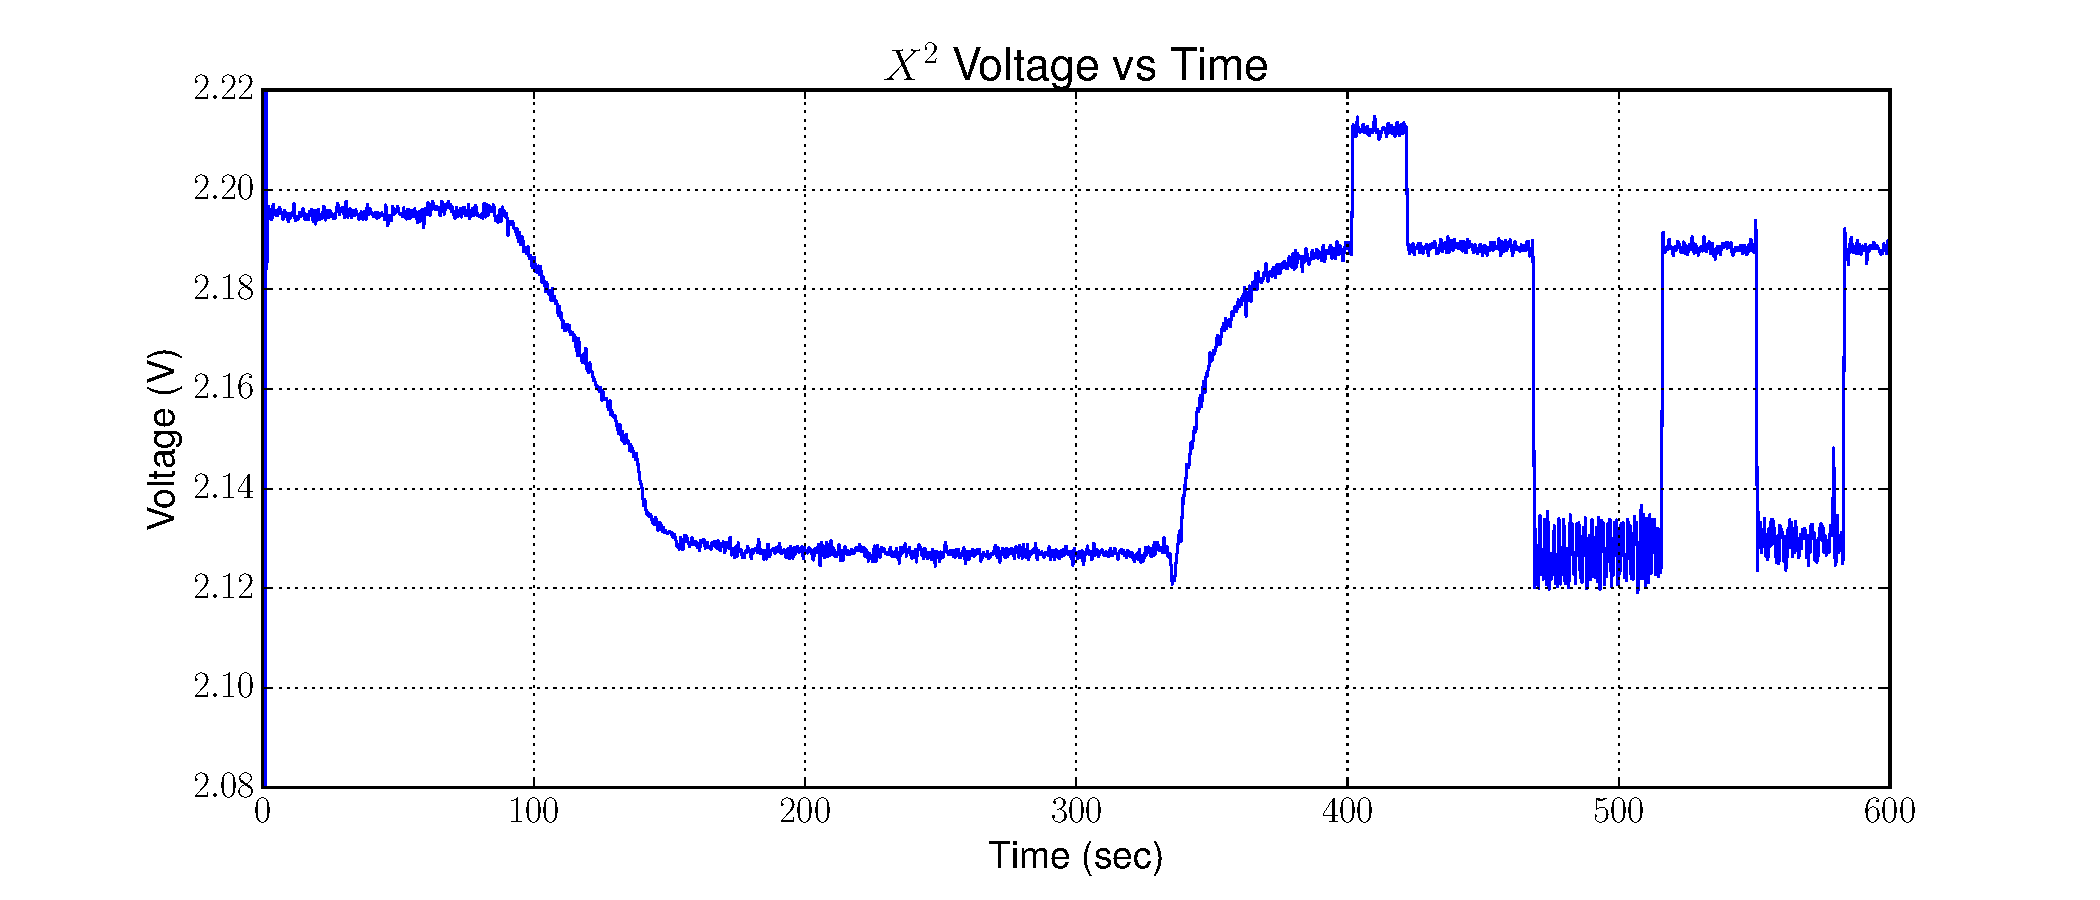
\includegraphics[width=\textwidth]{Experiments/Exp4/x2_voltage.pdf}
\isucaption{Graph showing the raw total power read from the square-law detector with an interfering signal.}
\label{x2_unfilt}
\end{figure}

We can clearly see in both the software defined radio and the square-law detector that there is an interfering signal.  If we now look at the spectrum view on the software defined radio, we can see the signal in questions which is at 1.405 GHz.  Figure \ref{spectrum_interfering} shows us what the software defined radio sees which is a spike at 1.405 GHz.  The square-law detector of course has no frequency information, so our only method to detect an interfering signal is by looking at the total power readings.  In our case there is elevated readings and we can see the spikes in the square-law data.  However, we do not know where in the spectrum the signal is at.

\begin{figure}[h!tb] \centering
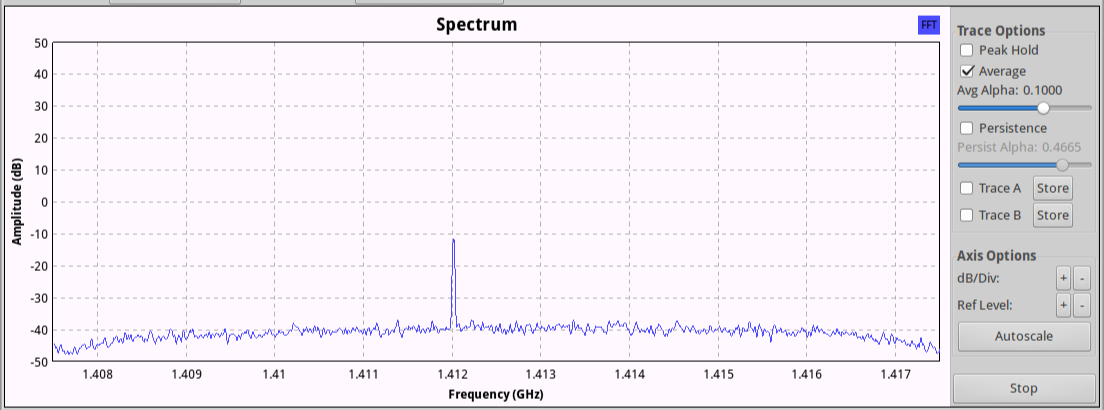
\includegraphics[width=\textwidth]{Images/spectrum_interference.png}
\isucaption{Image showing the spectrum view from the software defined radio}
\label{spectrum_interfering}
\end{figure}

Since we know where the offending signal is, we can now design our filter to filter out this signal.  In our GNURadio program we can specify both the frequency and the bandwidth our band-reject filter that we desire.  Ideally we want to keep the bandwidth of the filter as tight as possible to the offending signal but we also want to make sure our filter is effective in removing the signal.  Figure \ref{spectrum_filter} shows the spectrum display from the software defined radio with the filter now turned on and filtering the offending signal.

\begin{figure}[h!tb] \centering
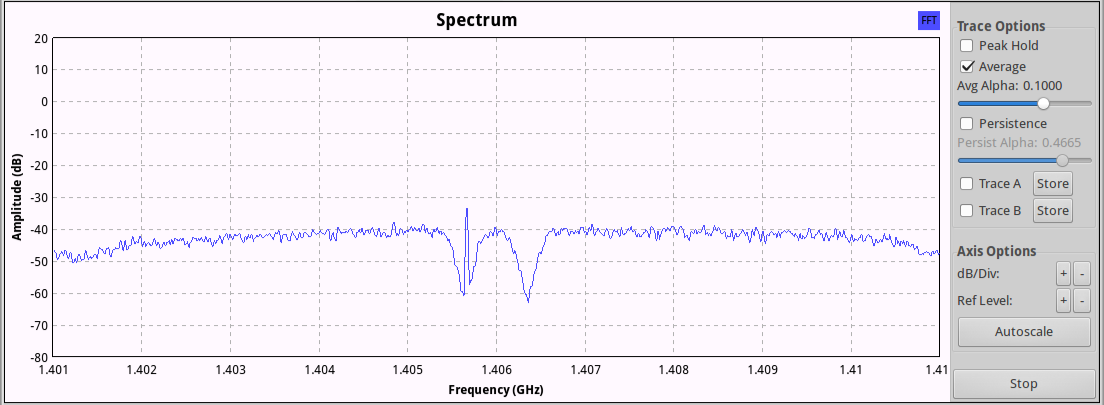
\includegraphics[width=\textwidth]{Images/spectrum_filter.png}
\isucaption{Image showing the software defined radio with the filter on and filtering the offending signal}
\label{spectrum_filter}
\end{figure}

Since we have now removed the offending signal, we will want to re-run our experiment and once again compare the difference between the software defined radio and the square law detector. We can begin by looking at the software defined radio total power readings.  In figure \ref{sdr_calib_filter} we can see a calibrated graph of the noise temperature seen by the software defined radio.  This graph is very similar to the graphs we expect from our total power radiometer.  However, we want to compare this to our square-law detector as well.  

\begin{figure}[h!tb] \centering
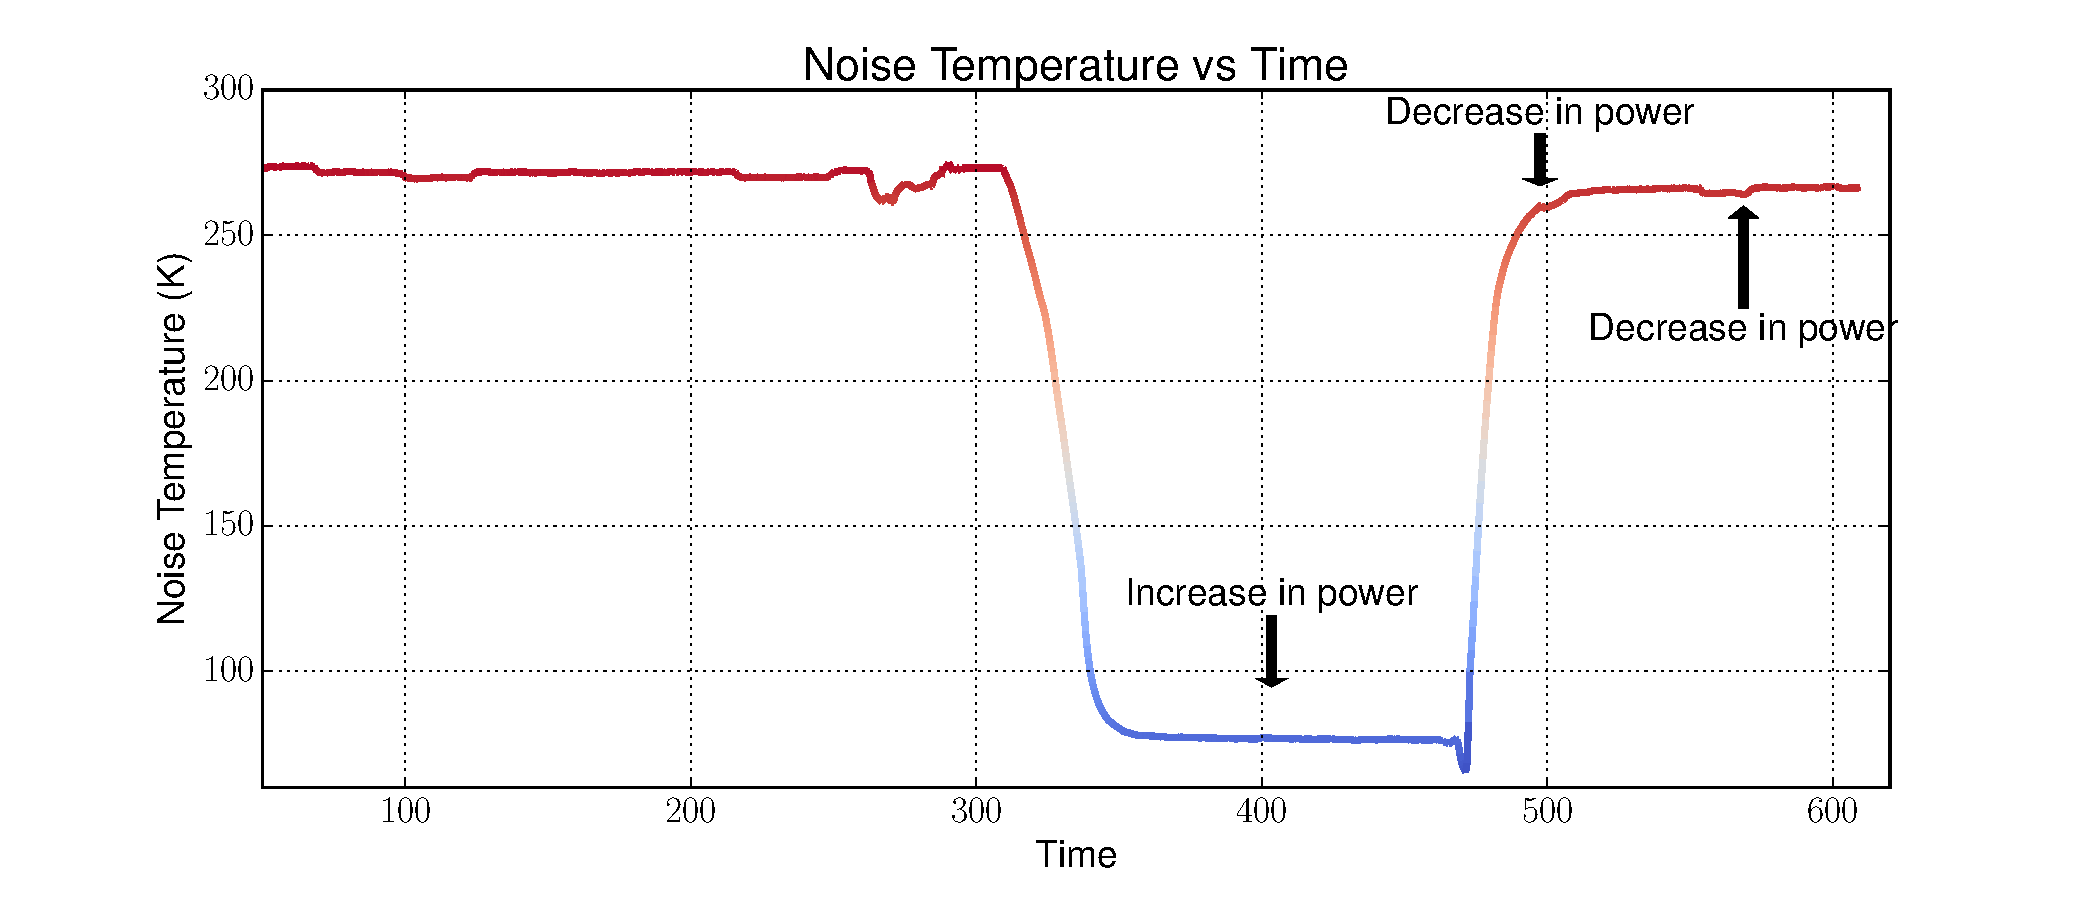
\includegraphics[width=\textwidth]{Experiments/Exp4/calib_filtered.pdf}
\isucaption{Graph showing the calibrated total power readings with the filter removing the offending signal}
\label{sdr_calib_filter}
\end{figure}

Figure \ref{filter_on} now shows both the software defined radio and the square-law detector calibrated total power readings.  In this graph you can see that the software defined radio is able to make normal readings where the square-law detector still shows the changes in amplitude which would make both calibration and obtaining useful data difficult.

\begin{figure}[h!tb] \centering
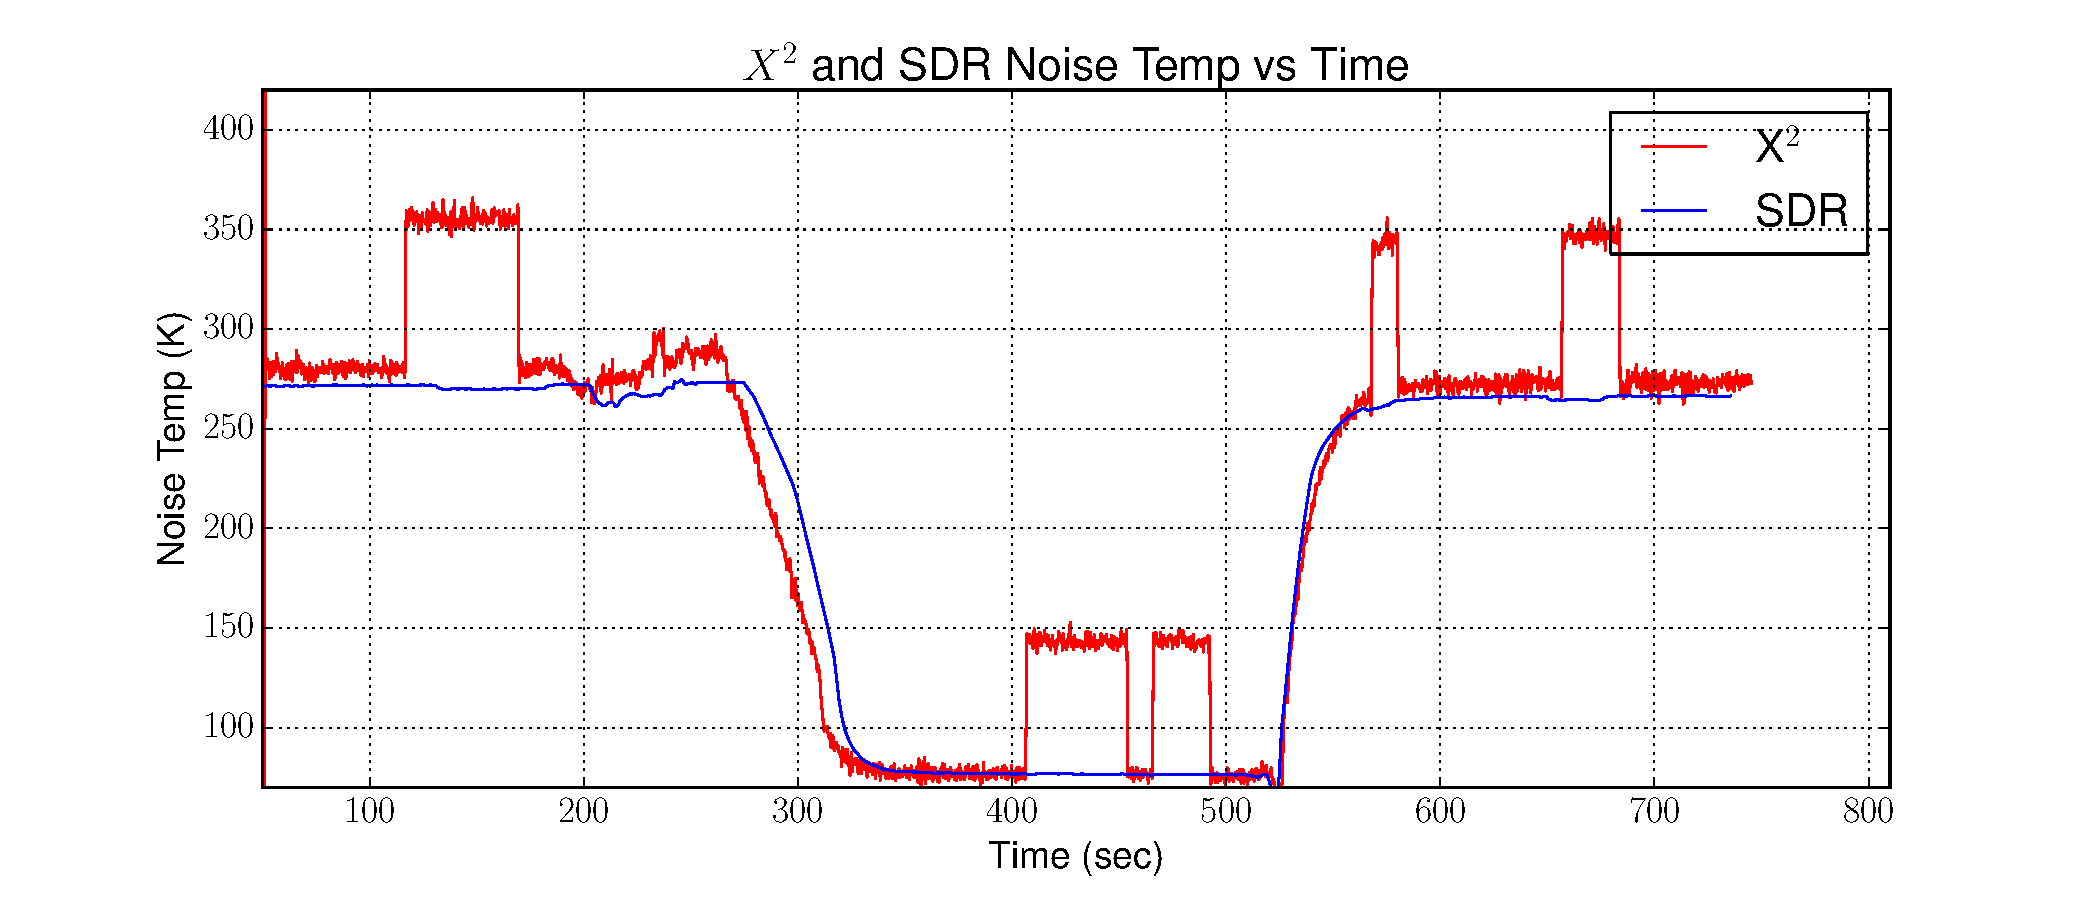
\includegraphics[width=\textwidth]{Experiments/Exp4/calib_filtered_both.pdf}
\isucaption{Image of the offending signal being filtered out by the SDR.  It can be seen that the signal is no longer visible.}
\label{filter_on}
\end{figure}

\emph{Filter delay.}  It should be noted that when doing data analysis with this data, that there will be some delay due to two factors.  First, there is a delay in the software defined radiometer due to the integrator that is used.  This creates a time delay as the integrator accumulates information and then settles.  We use fairly large integration times, usually in seconds so this can add a significant delay.  Second we do have a smaller delay in the decimation and low power filter also used in the software defined radiometer.  These are Finite Impulse Response (FIR) filters and thus have a delay given in equation \ref{FIR_delay}, where $N$ is the number of taps generated and $F_{s}$ is our sampling frequency, in our case 10 MHz.

\begin{equation}\label{FIR_delay}
\frac{(N - 1)}{(2*F_{s})}
\end{equation}

The taps value is generated by Python using the filter design program.  For this experiment, the taps generated was 18,181.  Taking that and our sampling rate into account, our FIR filter only delays the signal by 9 milliseconds.  

A final note on lining up the square-law detector information and the software defined radiometer data.  Both systems have a record function and must be started manually by the user.  They also run on separate computers.  Therefore, there is a human error that also gets introduced to the system as well.  This is usually no more than 1 or 2 seconds.  But in this experiment it was noted that there was a slightly longer delay between the two of about 4 seconds.  

\section{Experiment IV - Performance impact of interfering signal mitigation} \label{Exp4_results}
The goal of this experiment is to examine what affect adding a filter does to the performance of the radiometer.  This performance would be the same no matter what type of radiometer we use as a f

\subsection{Data Collected}
The data collected for this experiment is the data points collected in table \ref{exp4_data_power} and table \ref{exp4_datapoints}.  The remaining data is data generated from the equations outlined in this section.

\begin{table}[h!tb] \centering
\isucaption{Measured sensitivity and Bandwidth of Filter}
\label{exp4_data_power}
% Use: \begin{tabular{|lc|} to put table in a box
\begin{tabular}{lc} \hline
\textbf{rQ Value} & \textbf{Temperature (K)} \\ \hline
.139 & .125 \\
.141 & .250 \\
.143 & .500 \\
.147 & 1 \\
.153 & 2 \\
.166 & 3 \\
.181 & 4 \\
.195 & 5 \\
.234 & 6 \\
.252 & 7 \\
.318 & 8 \\
.450 & 9 \\
1.45 & 10 \\ \hline
\end{tabular}
\end{table}

\begin{table}[h!tb] \centering
\isucaption{Measured Total Power and Bandwidth of Signal}
\label{exp4_datapoints}
% Use: \begin{tabular{|lc|} to put table in a box
\begin{tabular}{lc} \hline
\textbf{rQ Value} & \textbf{Bandwidth (MHz)} \\ \hline
.003 & .125 \\
.006 & .250 \\
.012 & .500 \\
.025 & 1 \\
.050 & 2 \\
.071 & 3 \\
.101 & 4 \\
.125 & 5 \\
.140 & 6 \\
.170 & 7 \\
.200 & 8 \\
.230 & 9 \\
.250 & 10 \\ \hline
\end{tabular}
\end{table}

\subsection{Data Analysis}

For experiment four, we will look at the performance of a software defined radiometer when a filter is used and what impact that has.  Recall the following equation for $NE\Delta T$ from equation \ref{NEAT_EQ}.  Our sensitivity is based on the amount of noise we have from both the antenna or $T_{A}$ plus the addition of our system noise which is $T_{sys}$.  Finally our bandwidth of the signal, $\beta$ and our integration time, $\tau$, are the final factors that determine our $NE\Delta T$.

Our integration time is controllable, and can be set using the GUI panel for the software defined radio.  In a typical radiometer, we often do not have any control of the bandwidth.  It is often set by the mechanical bandwidth filters that are in place and the detection circuit to detect the noise power.  In a software defined radio radio we do have more control on bandwidth as we can change our sampling rate which in turns controls our bandwidth.  There is a limit as larger sampling rates require more data and processing bandwidth to process.  

Recall from experiment III in section \ref{Exp3_results} where we filtered out an offending signal.  While this allows us to filter out the offending signal and resume total power measurements, it comes at a cost of reducing the overall bandwidth available for power detection.  In this experiment we look at this and derived the following equation \ref{NEAT_FILTER}.

\begin{equation}\label{NEAT_FILTER}
NE\Delta T=\frac{T_{A}+T_{sys}}{\sqrt{(\beta - \beta_{filter})  \tau}}
\end{equation}

Since we are notching out a portion of the bandwidth in order to remove the offending signal, this also takes away that bandwidth for our total power detection.  The larger the filter, the more bandwidth that is subtracted from the total bandwidth available.  Equation \ref{NEAT_FILTER} accounts for this loss by subtracting the filter bandwidth from the total bandwidth.  

This equation now takes into account the subtraction of the filter.  The width of the band reject filter used then affects our $NE\Delta T$ and thus our performance of the radiometer.  

\begin{figure}[h!tb] \centering
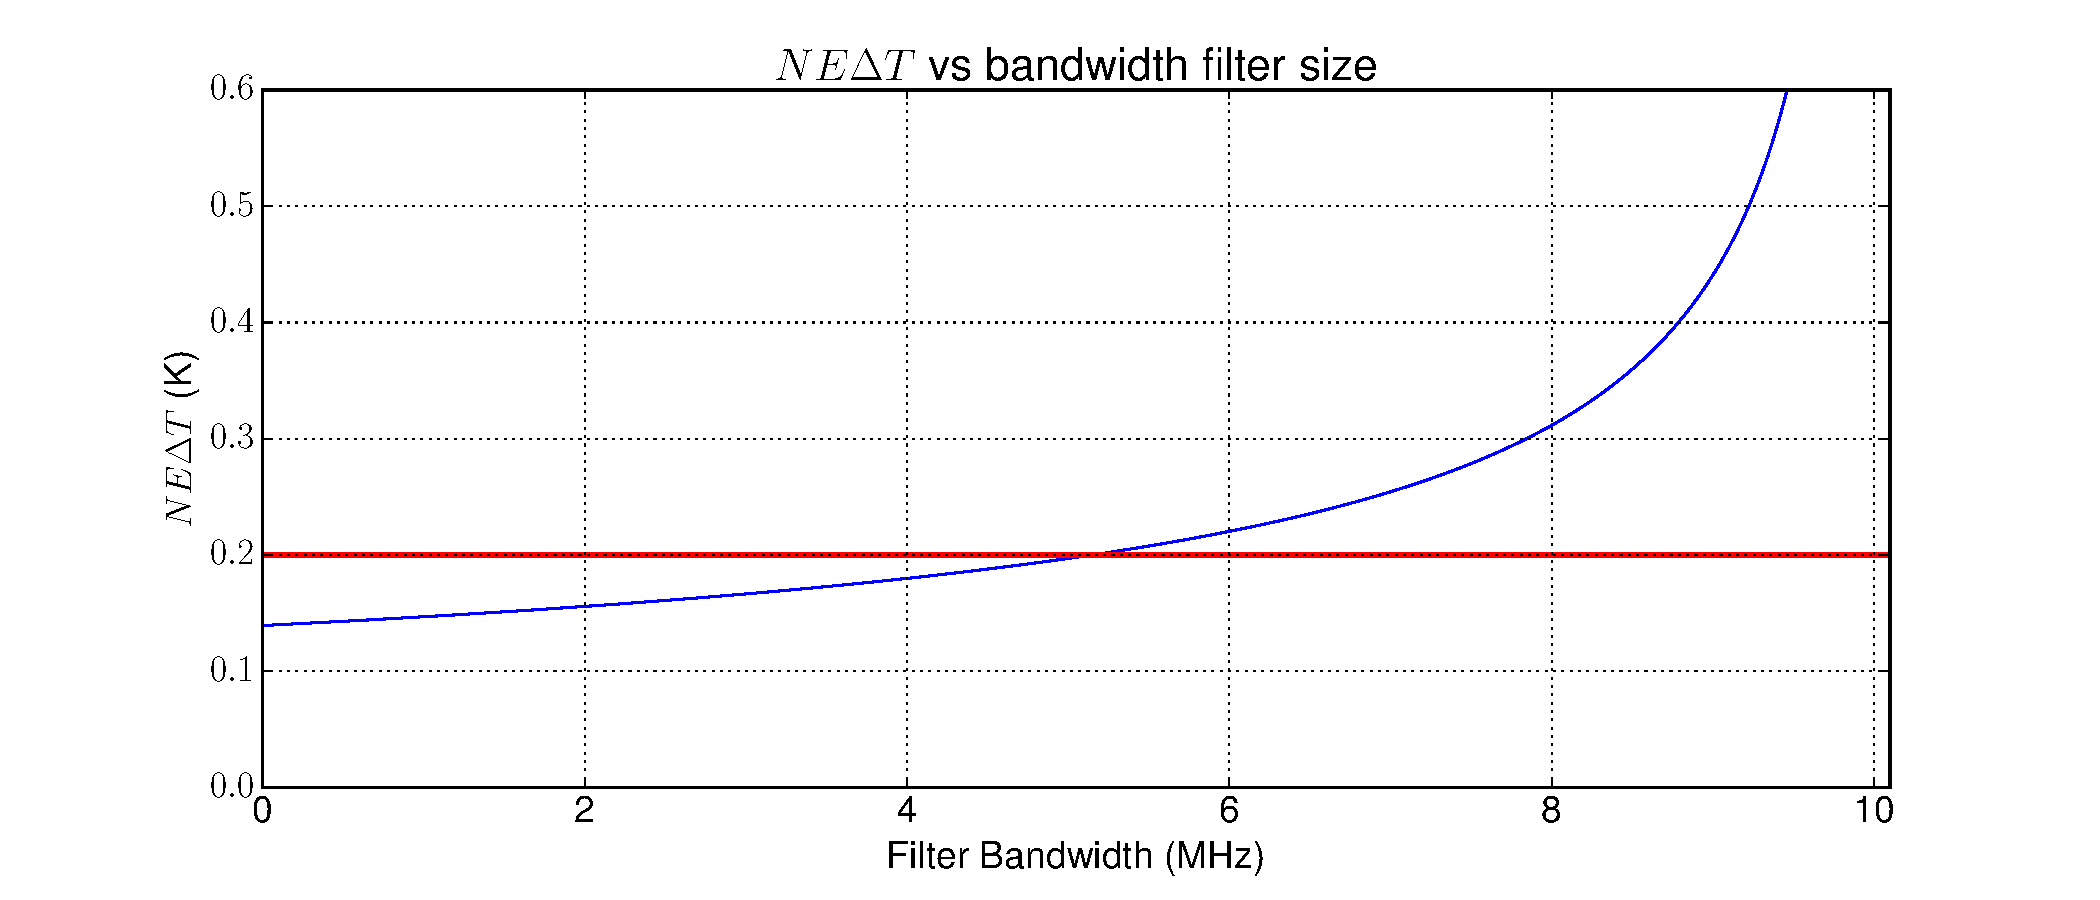
\includegraphics[width=\textwidth]{Experiments/Exp5/neatvsbw_plot.pdf}
\isucaption{Graph of the calculated $NE\Delta T$, the proposed limit for the sensitivity of the radiometer and the measured standard deviation compared to the bandwidth filter size.}
\label{neat_bw}
\end{figure}

We can graph the expected response of the $NE\Delta T$ by adjusting the values of $\beta_{fitler}$ to range from a narrowband filter, in our example 125 kHz all the way to 9.99 MHz or nearly all of the bandwidth.  Figure \ref{neat_bw} shows the expected exponential response of the $NE\Delta T$ as the size of the filter increases.  

Figure \ref{neat_bw} also shows measured standard deviation points for the software defined radiometer for set filter sizes.  These filter sizes and collected data is in table \ref{exp4_data_power}.  It can be seen in figure \ref{neat_bw} that there is a good correlation between the expected sensitivity of the radiometer and the measured sensitivity of the radiometer.

\begin{figure}[h!tb] \centering
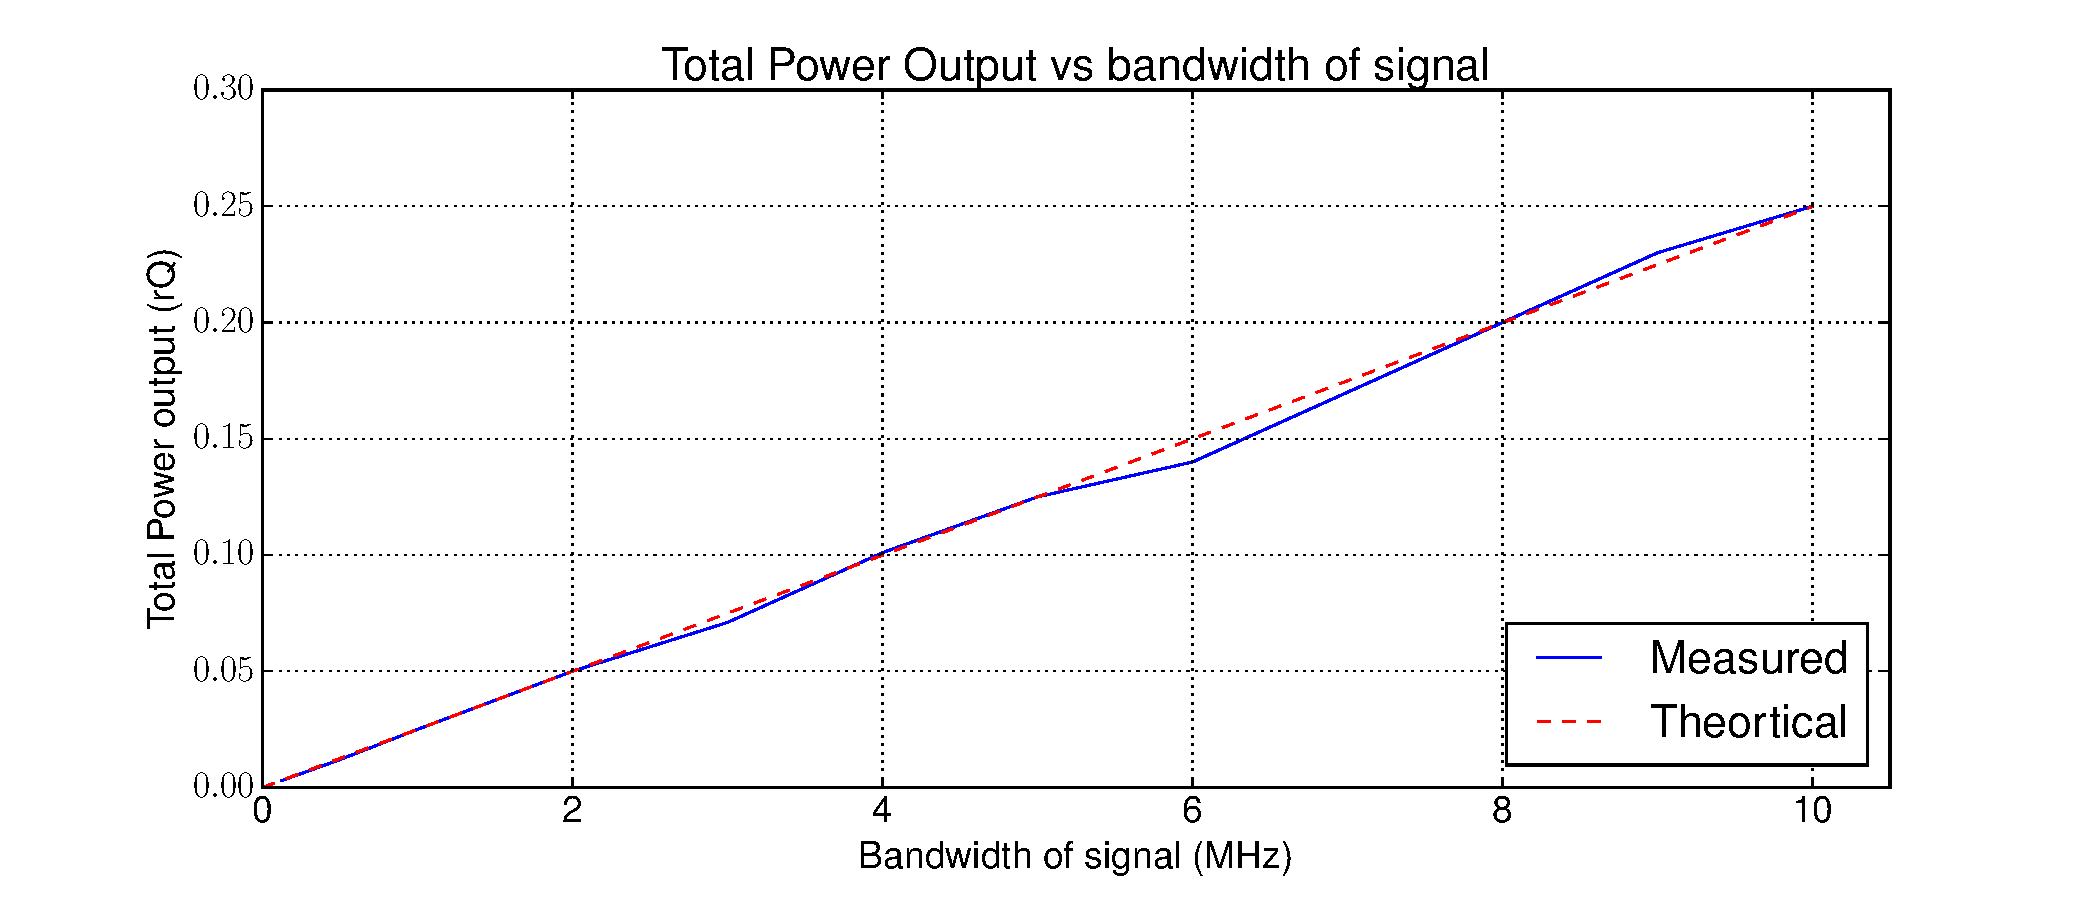
\includegraphics[width=\textwidth]{Experiments/Exp5/combined_plot.pdf}
\isucaption{Graph of the total power measured and theoretical power versus the bandwidth of the measured signal.}
\label{power_bw}
\end{figure}

Finally a line is added to figure \ref{neat_bw} to show a possible limit of when we may have filtered too much.  In this example a $NE\Delta T$ of 0.2 Kelvin is used.  In figure \ref{neat_bw} it can be seen that at about 5 MHz, our $NE\Delta T$ exceeds our threshold of 0.2 Kelvin.  This would mean that to meet this performance criteria, we would need to not filter out more than 5 MHz or about half of the available bandwidth.  

We can look at the relationship of the total power received as the bandwidth decreases.  Figure \ref{power_bw} shows us both the measured total power received and the expected total power received as the bandwidth of the filter increases.

The total power is calculated from equation \ref{eq:final_power} and is based on the total system noise, both from the antenna and generated from the system, the bandwidth and finally from the gain of the amplifiers used.  Our gain and noise temperatures are fixed, and in this experiment we use a system gain of 30 dB.  This represents the gain that we see with the three LNAs used minus any losses or attenuation placed in the RF chain.  What changes in this experiment is the amount of bandwidth.  Again, we can modify equation \ref{eq:final_power} by subtracting the filter bandwidth from the total bandwidth available and is shown in equation \ref{PWR_FILTER}.

\begin{equation}\label{PWR_FILTER}
P_{out}=k (\beta - \beta_{filter})G(T_{A}+T_{N})
\end{equation}

To compare this theoretical power to the actual power measured, we collected the rQ values by once again creating set filter sizes and then measuring the rQ value.  These values can be found in table \ref{exp4_datapoints} and are added to figure \ref{power_bw} as the dots indicated on the graph.  This also shows a very good correlation between the expected total power received and the measured total power received for experiment four.

%---------------------------------------------------------------

\section{Benefits to Software Defined Radio Radiometer}
A study was conducted on what benefits a software defined radio radiometer would have over a more traditional radiometer.  This was focused on looking at three main areas; cost, weight and size, and the value a SDR radiometer can add over traditional radiometers.

\subsection{Cost Benefits}
Software defined radios have become more commonplace in recent years and this has generated a number of Commercial Off The Shelf (COTS) solutions.  A COTS solution is often a lower cost solution due to the mass manufacturing that takes place.  This has driven the cost of many SDRs to under one thousand dollars while still having excellent performance characteristics.  The N200 SDR purchased for this research cost fifteen hundred dollars and the daughter-board cost one hundred and fifty dollars approximately.  Other software defined radios however have come out on the market since then.  Ettus for example has some that are below one thousand dollars and the author has also obtained the HackRF One SDR that now sells for three hundred dollars.  The main difference with the different software defined radios on the market is with both the resolution, or how many bits the ADC is, and the bandwidth they are able to handle.

\begin{table}[h!tb] \centering
\isucaption{Cost Analysis}
\label{cost_table}
% Use: \begin{tabular{|lcc|} to put table in a box
\begin{tabular}{lcc} \hline
\textbf{Device} & \textbf{Quantity} & \textbf{Cost} \\ \hline
\textbf{SDR Solution}& & \\ \hline
N200 SDR & 1 & \$1515 \\
LNA at \$60 ea. & 3 & \$180 \\
DBSRX2 Daughter-board & 1 & \$152 \\
GNURadio & 1 & \$0 \\ \hline
Total & & \$1847 \\ \hline
\textbf{ISU Radiometer} \\ \hline
LNA, FPGA, ADC, Microcontroller and power supplies & 1 & \$10,000\tablefootnote{Purchase price in 2005} \\ \hline
\textbf{Commercial Off the Shelf Unit}\\ \hline
Spectracyber 1420 MHz Hydrogen Line Spectrometer & 1 & \$2,650 \\ \hline

\end{tabular}
\end{table}

As seen in table \ref{cost_table}, even the higher cost Ettus research equipment is a lower cost option than the custom built ISU radiometer purchased from University of Michigan and even a comparable off the shelf radiometer.  It should be noted that the radiometer from the University of Michigan is also a dual polarization radiometer so there are two RF front ends and two ADCs that feed into a FPGA board.  It would be quite easy to add dual polarization to the Ettus N200 SDR as it does support two daughter-boards.  This would increase the cost to \$2,179 for the additional LNAs and daughter-board.

The largest cost benefit is that key components that you find in a radiometer, the filters and square-law detector can now be all done in software instead of needed additional equipment.  The system is also much more frequency agile, which means it can work on a broader range of frequencies than most traditional radiometers with very little change in hardware and in some cases may require no change in hardware.  Some of this does depend on the SDR hardware however.  The Ettus N200 for example uses daughter-boards to provide the RF interface.  While these boards provide a high quality in the RF signal, it does come at a cost and are usually designed for certain bands of frequencies.  Other low cost SDRs however are also very wide range in the frequencies they will work in.  The HackRF for example works from 10 MHz to 6 GHz, but does so at the cost of lower resolution, less gain in its front end and a lower bandwidth that it can handle.

\subsection{Weight and component size benefits}

A typical radiometer has many components that are involved in the design of the radiometer.  This includes filters, LNAs and the power detection or square-law detector used.  These components add both weight, size and costs to the radiometer.  A software defined radio however digitizes the signal and we are able to replace the filters and square-law detector with their software equivalent.  While a software defined radio does add both the ADC and usually a FPGA to do the processing on the signal, advances in semiconductor technology has continued to shrink these components.  These components are also lighter than the filters often used in radiometers.

\begin{table}[h!tb] \centering
\isucaption{Weight Analysis}
\label{weight_table}
% Use: \begin{tabular{|lcc|} to put table in a box
\begin{tabular}{lc} \hline
\textbf{Device} & \textbf{Mass} \\ \hline
\textbf{SDR Solution} & \\ \hline
N200 SDR & 1.2 kg \\
LNA at .03 kg ea & .09 kg \\
DBSRX2 Daughter-board & .1 kg \\ \hline
Total & 1.39 kg \\ \hline
\textbf{ISU Radiometer} \\ \hline
LNA, FPGA, ADC, Microcontroller and power supplies & 22.7 kg \\ \hline
\textbf{Commercial Off the Shelf Unit}\\ \hline
Spectracyber 1420 MHz Hydrogen Line Spectrometer & 6 kg\tablefootnote{Estimated, no data available} \\ \hline

\end{tabular}
\end{table}

Size is another benefit as since semiconductor technology has continued to shrink components.  Again, since items like the filters and square-law detector are removed and done in software this helps to reduce the overall size.  

\subsection{Value added benefits}

A software defined radio radiometer adds additional value for two reasons.  One, it is able to work with both frequency and magnitude where most radiometers do not.  This allows for additional analysis on the signal and can help identify issues such as an interfering signal that was demonstrated in this thesis.  

Second, we are able to have an agile system that is able to adapt to changing conditions with very little or no change to hardware.  Different types of radiometers can be implemented such as a Dicke radiometer, dual polarization radiometer or a radiometer that can perform Stokes parameters.  In addition, since we have both frequency and power information we can create a system that is able to adapt to changing conditions such as dealing with an interfering signal.  

\section{Disadvantages of a SDR Radiometer}
Although we have outlined a number of advantages of using a COTS SDR Radiometer and how a SDR can add additional value to the radiometer system, there are some disadvantages to a SDR Radiometer.

\subsection{Power Consumption}
One of the largest drawbacks to a SDR radiometer can be in the power consumption of the SDR.  With the move to perform functions such as power detection and filtering we now require additional computational power to perform these tasks.  With those computational cycles additional power is now required.  The use of FPGAs and SoC however can help to minimize these power concerns as they are more efficient than using a full scale x86 based processor and on board computer system.  

Power and CPU requirements also increase as we add additional functionality such as filtering an offending signal.  While these additions may not require additional hardware, it can require additional processor or computational requirements.  This will cause additional strain on the processor and also in the memory requirements for the SDR as well.

\subsection{Bandwidth constraints}
While SDR technology has advanced, bandwidth is still a constraint that affects SDRs and in turn a SDR Radiometer.  Bandwidth plays a critical role in the radiometer's sensitivity as explained in this thesis, therefore the fact that many SDRs are limited in bandwidth does create a disadvantage.  In many cases this bottleneck takes place in both the transport and processing of large bandwidth systems.  This also relates to the power consumption disadvantage since larger bandwidth also means requiring additional computational cycles as well.  

In contrast, a square-law detector usually has a very large bandwidth, as much as one gigahertz, and is why we usually need to filter to the frequency band of interest.  

\section{Results Summary}


%----------------------------------------------------------
% End of Chapter 6.  Anything below this is extra information

%The data collected was then graphed using Excel.  The graph shown in \ref{adl5902_linear} shows that the ADL5902 has a linear output and matches the expected value based on the input.  

%\begin{figure}[h!tb] \centering
%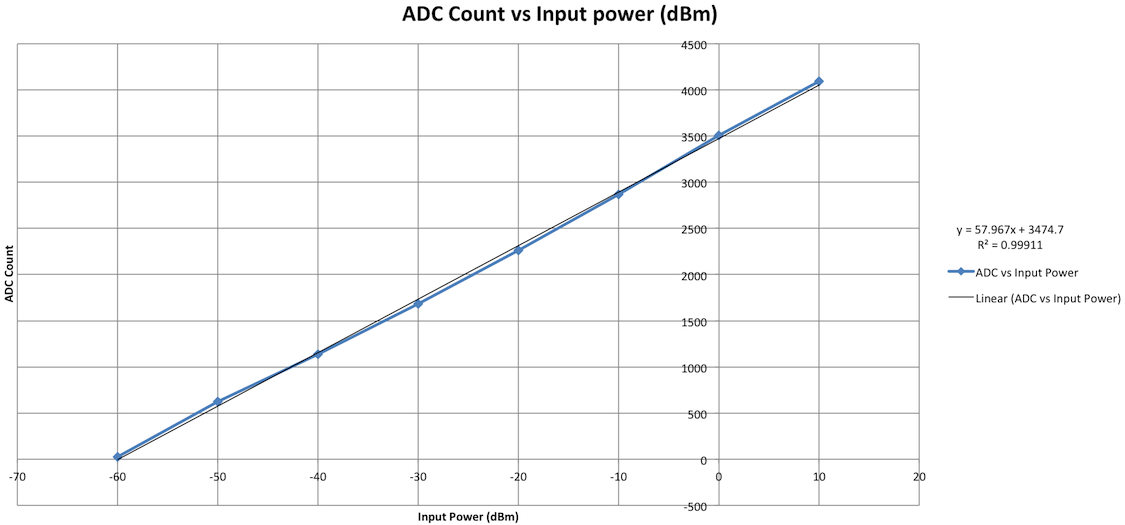
\includegraphics[width=\textwidth]{Images/Linearsquarelaw}
%\isucaption{Graph showing the linearity of the ADL5902}
%\label{adl5902_linear}
%\end{figure}

%Once it was confirmed the ADL5902 does in fact have a linear response, we then looked at ways to work with the ADL5902.  The graph above was generated using Analog Devices program that talked to the Blackfin processor on the daughter-board.  However, the information for talking to the Blackfin is proprietary.  Therefore, the daughter-board was removed for future tests and instead we used the USB-6009 data acquisition board to read the raw analog voltages from the ADL5902.  This information was then stored later for additional analysis.  

%Matlab is one tool we can use to process the information that is stored by GNURadio.  Appendix A contains the Matlab source that will read the total power file generated by GNURadio.  It then calculates information such as the NE$\Delta$T and the calibration points based on the user input.  We can also use Matalb to graph this information as well.

%While Matlab is one tool, other tools can be used.  Python for example is also capable of reading in these files and when paired with NumPy and SciPy can be used to perform analysis on the data as well [\cite{Uengtrakul}].  In addition, the open source mathematical program Octave should also be able to read and work with these files.  For this thesis both Matlab and Python was used to provide analysis on the data.  

%Most of the graphs generated in this thesis was generated using iPython notebooks.  IPython notebooks uses Python but allows it to be executed in a web browser either locally or on a server.  Using iPython notebooks however also allows us to add additional information using Markdown and basic HTML.  This allowed the author to paint a complete picture of the experimental results illustrating pictures of the setup and the code and steps used to analyze the data.  You can find these notebooks on the author's Github site and can use NBViewer to view them.  An example link is \href{http://nbviewer.ipython.org/github/matgyver/Radiometer-SDR-Thesis/blob/master/Experiments/Exp1/radiometer_experiment_1.ipynb}.